%\documentclass[review]{elsarticle}
\documentclass[final,5p]{elsarticle}
%\documentclass[authoryear]{elsarticle}

\usepackage{xcolor}
\usepackage[colorlinks, allcolors=black]{hyperref}
\usepackage{lineno,amssymb,bm,amsmath,caption,subcaption,booktabs,rotating,tikz,cleveref,gensymb}
\usetikzlibrary{decorations.pathreplacing}
\usepackage[percent]{overpic}
\usepackage[export]{adjustbox}
\usepackage[normalem]{ulem}
\usepackage{dvmacros}
%\modulolinenumbers[100]
\nolinenumbers
\newcommand\hl[1]{%
  \bgroup
  \hskip0pt\color{black!80!black}%
  #1%
  \egroup
}
\let\linenumbers\nolinenumbers\nolinenumbers
\journal{Medical Image Analysis}

%%%%%%%%%%%%%%%%%%%%%%%%%%%%%%%%%%
%% Elsevier bibliography styles %%
%%%%%%%%%%%%%%%%%%%%%%%%%%%%%%%%%%

%\usepackage{numcompress}
%\bibliographystyle{model3-num-names}
\bibliographystyle{model4-names}
\biboptions{authoryear}
%\bibliographystyle{elsarticle-num}
%\bibliographystyle{elsarticle-num-names}
%\bibliographystyle{elsarticle-harv}
%\bibliographystyle{plain}
%\bibliographystyle{alpha}
%\bibliographystyle{amsplain}
%\bibliographystyle{amsalpha}

\usepackage{ctex}

%%%%%%%%%%%%%%%%%%%%%%%%%%%%%%%%%%%%%%%%%%%%%%%%%%%%%%%%%%%%%%%%%%%%%%%%%%%%%%%%


\begin{document}

%%%%%%%%%%
% MICCAI %
%%%%%%%%%%

% Jaccard

\newcommand{\ACDCONJLVBP}{0.912}
\newcommand{\ACDCONJRVBP}{0.852}
\newcommand{\ACDCONJLVMY}{0.803}

\newcommand{\ACDCFINJLVBP}{0.896}
\newcommand{\ACDCFINJRVBP}{0.832}
\newcommand{\ACDCFINJLVMY}{0.826}

\newcommand{\ACDCFIOJLVBP}{0.869}
\newcommand{\ACDCFIOJRVBP}{0.784}
\newcommand{\ACDCFIOJLVMY}{0.775}

% Dice

\newcommand{\ACDCONDLVBP}{0.954}
\newcommand{\ACDCONDRVBP}{0.920}
\newcommand{\ACDCONDLVMY}{0.891}

\newcommand{\ACDCFINDLVBP}{0.945}
\newcommand{\ACDCFINDRVBP}{0.908}
\newcommand{\ACDCFINDLVMY}{0.905}

\newcommand{\ACDCFIODLVBP}{0.930}
\newcommand{\ACDCFIODRVBP}{0.879}
\newcommand{\ACDCFIODLVMY}{0.873}

% Data Set

\newcommand{\SpacingMU}{1.3}
\newcommand{\SpacingSD}{0.2}
\newcommand{\MatrixMU}{253.53}
\newcommand{\MatrixSD}{46.73}

\newcommand{\NumPtC}{21}
\newcommand{\NumPtO}{42}
\newcommand{\NumPtT}{63}
\newcommand{\N}{256}
\newcommand{\NumFramesMin}{20}
\newcommand{\NumFramesMax}{50}

% Cross Validation
\newcommand{\NumFolds}{3}
\newcommand{\NumImFoldA}{4477}
\newcommand{\NumImFoldB}{4750}
\newcommand{\NumImFoldC}{4625}

% Architecture
\newcommand{\networkmomentum}{0.9}
\newcommand{\weightdecay}{10^{-4}}
%\newcommand{\trainablekernels}{128}

% Augmentation
\newcommand{\AugTrans}{0.15}
\newcommand{\AugRot}{\hl{15}}
\newcommand{\AugZoom}{0.15}

\newcommand{\AUC}{0.992}

\newcommand{\SAXAlvendCGlobalMu}{-24.9}
\newcommand{\SAXAlvendCGlobalSd}{7.8}
\newcommand{\SAXAlvendOGlobalMu}{-29.8}
\newcommand{\SAXAlvendOGlobalSd}{13.6}
\newcommand{\SAXAlvendpGlobal}{NS}
\newcommand{\SAXAlvepiCGlobalMu}{-10.3}
\newcommand{\SAXAlvepiCGlobalSd}{3.5}
\newcommand{\SAXAlvepiOGlobalMu}{-11.8}
\newcommand{\SAXAlvepiOGlobalSd}{13.7}
\newcommand{\SAXAlvepipGlobal}{NS}
\newcommand{\SAXBlvendCGlobalMu}{-28.0}
\newcommand{\SAXBlvendCGlobalSd}{4.1}
\newcommand{\SAXBlvendOGlobalMu}{-28.6}
\newcommand{\SAXBlvendOGlobalSd}{6.3}
\newcommand{\SAXBlvendpGlobal}{NS}
\newcommand{\SAXBlvepiCGlobalMu}{-13.2}
\newcommand{\SAXBlvepiCGlobalSd}{3.1}
\newcommand{\SAXBlvepiOGlobalMu}{-10.6}
\newcommand{\SAXBlvepiOGlobalSd}{3.5}
\newcommand{\SAXBlvepipGlobal}{<0.01}
\newcommand{\SAXElvendCGlobalMu}{-24.7}
\newcommand{\SAXElvendCGlobalSd}{4.4}
\newcommand{\SAXElvendOGlobalMu}{-28.7}
\newcommand{\SAXElvendOGlobalSd}{6.0}
\newcommand{\SAXElvendpGlobal}{<0.05}
\newcommand{\SAXElvepiCGlobalMu}{-8.9}
\newcommand{\SAXElvepiCGlobalSd}{2.7}
\newcommand{\SAXElvepiOGlobalMu}{-7.7}
\newcommand{\SAXElvepiOGlobalSd}{3.2}
\newcommand{\SAXElvepipGlobal}{NS}

%%%%%%%%%%%%%%%%%%%%%%%%%%%%%%%
%% Channel 1, Atrous False
%%%%%%%%%%%%%%%%%%%%%%%%%%%%%%%
%
%\newcommand{\AAMZe}{0.846}
%\newcommand{\AALZe}{0.798}
%\newcommand{\AAHZe}{0.879}
%\newcommand{\ASMZe}{0.851}
%\newcommand{\ASLZe}{0.801}
%\newcommand{\ASHZe}{0.884}
%\newcommand{\AHMZe}{0.831}
%\newcommand{\AHLZe}{0.778}
%\newcommand{\AHHZe}{0.866}
%\newcommand{\AVMZe}{0.848}
%\newcommand{\AVLZe}{0.810}
%\newcommand{\AVHZe}{0.876}
%
%%%%%%%%%%%%%%%%%%%%%%%%%%%%%%%
%% Channel 1, Atrous True
%%%%%%%%%%%%%%%%%%%%%%%%%%%%%%%
%
%\newcommand{\BAMZe}{0.846}
%\newcommand{\BALZe}{0.799}
%\newcommand{\BAHZe}{0.879}
%\newcommand{\BSMZe}{0.851}
%\newcommand{\BSLZe}{0.800}
%\newcommand{\BSHZe}{0.885}
%\newcommand{\BHMZe}{0.833}
%\newcommand{\BHLZe}{0.789}
%\newcommand{\BHHZe}{0.865}
%\newcommand{\BVMZe}{0.847}
%\newcommand{\BVLZe}{0.808}
%\newcommand{\BVHZe}{0.876}
%
%%%%%%%%%%%%%%%%%%%%%%%%%%%%%%%
%% Channel 2, Atrous False
%%%%%%%%%%%%%%%%%%%%%%%%%%%%%%%
%
%\newcommand{\CAMZe}{0.848}
%\newcommand{\CALZe}{0.799}
%\newcommand{\CAHZe}{0.879}
%\newcommand{\CSMZe}{0.853}
%\newcommand{\CSLZe}{0.800}
%\newcommand{\CSHZe}{0.885}
%\newcommand{\CHMZe}{0.833}
%\newcommand{\CHLZe}{0.783}
%\newcommand{\CHHZe}{0.867}
%\newcommand{\CVMZe}{0.846}
%\newcommand{\CVLZe}{0.810}
%\newcommand{\CVHZe}{0.873}
%
%%%%%%%%%%%%%%%%%%%%%%%%%%%%%%%
%% Channel 2, Atrous True
%%%%%%%%%%%%%%%%%%%%%%%%%%%%%%%
%
%\newcommand{\DAMZe}{0.846}
%\newcommand{\DALZe}{0.797}
%\newcommand{\DAHZe}{0.880}
%\newcommand{\DSMZe}{0.852}
%\newcommand{\DSLZe}{0.795}
%\newcommand{\DSHZe}{0.885}
%\newcommand{\DHMZe}{0.830}
%\newcommand{\DHLZe}{0.781}
%\newcommand{\DHHZe}{0.862}
%\newcommand{\DVMZe}{0.849}
%\newcommand{\DVLZe}{0.815}
%\newcommand{\DVHZe}{0.878}


\newcommand{\AALZe}{0.783}
\newcommand{\AAMZe}{0.834}
\newcommand{\AAHZe}{0.871}
\newcommand{\ASLZe}{0.789}
\newcommand{\ASMZe}{0.843}
\newcommand{\ASHZe}{0.880}
\newcommand{\AHLZe}{0.765}
\newcommand{\AHMZe}{0.819}
\newcommand{\AHHZe}{0.855}
\newcommand{\AVLZe}{0.788}
\newcommand{\AVMZe}{0.831}
\newcommand{\AVHZe}{0.863}
\newcommand{\BALZe}{0.793}
\newcommand{\BAMZe}{0.841}
\newcommand{\BAHZe}{0.876}
\newcommand{\BSLZe}{0.800}
\newcommand{\BSMZe}{0.848}
\newcommand{\BSHZe}{0.884}
\newcommand{\BHLZe}{0.780}
\newcommand{\BHMZe}{0.831}
\newcommand{\BHHZe}{0.861}
\newcommand{\BVLZe}{0.787}
\newcommand{\BVMZe}{0.832}
\newcommand{\BVHZe}{0.864}
\newcommand{\BALOn}{0.819}
\newcommand{\BAMOn}{0.857}
\newcommand{\BAHOn}{0.885}
\newcommand{\BSLOn}{0.820}
\newcommand{\BSMOn}{0.862}
\newcommand{\BSHOn}{0.891}
\newcommand{\BHLOn}{0.812}
\newcommand{\BHMOn}{0.845}
\newcommand{\BHHOn}{0.871}
\newcommand{\BVLOn}{0.822}
\newcommand{\BVMOn}{0.856}
\newcommand{\BVHOn}{0.882}
\newcommand{\CALZe}{0.792}
\newcommand{\CAMZe}{0.841}
\newcommand{\CAHZe}{0.875}
\newcommand{\CSLZe}{0.797}
\newcommand{\CSMZe}{0.849}
\newcommand{\CSHZe}{0.883}
\newcommand{\CHLZe}{0.779}
\newcommand{\CHMZe}{0.830}
\newcommand{\CHHZe}{0.861}
\newcommand{\CVLZe}{0.793}
\newcommand{\CVMZe}{0.830}
\newcommand{\CVHZe}{0.863}
\newcommand{\CALOn}{0.816}
\newcommand{\CAMOn}{0.856}
\newcommand{\CAHOn}{0.884}
\newcommand{\CSLOn}{0.820}
\newcommand{\CSMOn}{0.862}
\newcommand{\CSHOn}{0.890}
\newcommand{\CHLOn}{0.804}
\newcommand{\CHMOn}{0.843}
\newcommand{\CHHOn}{0.869}
\newcommand{\CVLOn}{0.818}
\newcommand{\CVMOn}{0.855}
\newcommand{\CVHOn}{0.883}
\newcommand{\CALTw}{0.816}
\newcommand{\CAMTw}{0.857}
\newcommand{\CAHTw}{0.885}
\newcommand{\CSLTw}{0.819}
\newcommand{\CSMTw}{0.862}
\newcommand{\CSHTw}{0.890}
\newcommand{\CHLTw}{0.805}
\newcommand{\CHMTw}{0.844}
\newcommand{\CHHTw}{0.869}
\newcommand{\CVLTw}{0.819}
\newcommand{\CVMTw}{0.857}
\newcommand{\CVHTw}{0.884}
\newcommand{\DALZe}{0.797}
\newcommand{\DAMZe}{0.844}
\newcommand{\DAHZe}{0.877}
\newcommand{\DSLZe}{0.798}
\newcommand{\DSMZe}{0.851}
\newcommand{\DSHZe}{0.886}
\newcommand{\DHLZe}{0.781}
\newcommand{\DHMZe}{0.832}
\newcommand{\DHHZe}{0.861}
\newcommand{\DVLZe}{0.804}
\newcommand{\DVMZe}{0.842}
\newcommand{\DVHZe}{0.869}
\newcommand{\DALOn}{0.819}
\newcommand{\DAMOn}{0.856}
\newcommand{\DAHOn}{0.884}
\newcommand{\DSLOn}{0.821}
\newcommand{\DSMOn}{0.862}
\newcommand{\DSHOn}{0.890}
\newcommand{\DHLOn}{0.805}
\newcommand{\DHMOn}{0.839}
\newcommand{\DHHOn}{0.868}
\newcommand{\DVLOn}{0.828}
\newcommand{\DVMOn}{0.858}
\newcommand{\DVHOn}{0.884}
\newcommand{\DALTw}{0.821}
\newcommand{\DAMTw}{0.858}
\newcommand{\DAHTw}{0.886}
\newcommand{\DSLTw}{0.822}
\newcommand{\DSMTw}{0.863}
\newcommand{\DSHTw}{0.892}
\newcommand{\DHLTw}{0.811}
\newcommand{\DHMTw}{0.843}
\newcommand{\DHHTw}{0.870}
\newcommand{\DVLTw}{0.831}
\newcommand{\DVMTw}{0.860}
\newcommand{\DVHTw}{0.886}
\newcommand{\DALTh}{0.821}
\newcommand{\DAMTh}{0.858}
\newcommand{\DAHTh}{0.886}
\newcommand{\DSLTh}{0.822}
\newcommand{\DSMTh}{0.863}
\newcommand{\DSHTh}{0.892}
\newcommand{\DHLTh}{0.811}
\newcommand{\DHMTh}{0.843}
\newcommand{\DHHTh}{0.869}
\newcommand{\DVLTh}{0.830}
\newcommand{\DVMTh}{0.859}
\newcommand{\DVHTh}{0.886}
\newcommand{\MillionsOfParamsA}{7.0}
\newcommand{\MillionsOfParamsB}{3.5}
\newcommand{\MillionsOfParamsC}{4.5}
\newcommand{\MillionsOfParamsD}{5.5}

\begin{frontmatter}

\title{\omeganet{} \hl{(Omega-Net)}: 利用深度卷积神经网络进行全自动的多切面的心脏 MR 图像检测、取向和定位}

\author[oxford,nih,tufts]{Davis M. Vigneault\corref{mycorrespondingauthor}}
\ead{davis.vigneault@gmail.com}

\author[oxford]{Weidi Xie\corref{mycorrespondingauthor}}
\author[brigham]{Carolyn Y. Ho}
\author[wisc]{David A. Bluemke}
\author[oxford]{J. Alison Noble}

\address[oxford]{Institute of Biomedical Engineering, Department of Engineering, University of Oxford}
\address[nih]{Department of Radiology and Imaging Sciences, Clinical Center, National Institutes of Health}
\address[tufts]{Tufts University School of Medicine, Sackler School of Graduate Biomedical Sciences}
\address[brigham]{Cardiovascular Division, Brigham and Women's Hospital}
\address[wisc]{University of Wisconsin-Madison, School of Medicine and Public Health}

\cortext[mycorrespondingauthor]{这些作者对本文有同等贡献.}

\begin{abstract}


二维静态图像序列(SSFP, steady state free precession)的左心和四腔心分割是进行其他各种分析之前重要的一步.
考虑到对比度、外观、方向、病人心脏位置、临床切面、扫描仪以及协议的不同,心脏的全自动语义分割是一个非常难以解决的问题.
本文中,我们提出一个新的卷积神经网络(CNN),它可以同时完成定位,变换到典型方向,以及语义分割.
首先,对输入图像进行一个\hl{初始}分割;然后在初始分割过程中学习到特征会用来预测将图像变换到一个典型方向所需的参数;最后,对变换后的图像进行细分割.
在这个工作中,我们训练了不同深度的 \omeganet 来检测五个类别(短轴切面,SA;四腔心切面,4C;两腔心切面,2C),而不给出任何的先验知识.
这个工作比之前的工作更加有挑战性.
网络训练使用的数据来自肥厚型心肌病受试者(HCM, $N = \NumPtO{}$)和健康受试者($N = \NumPtC{}$).
网络的性能比起没有定位和方向信息的 \UNet{} 比起来好很多,IoU 为 $0.858$ vs $0.834$.
此外,为了与其他工作进行对比,我们从头开始,在 2017 MICCAI 自动心脏诊断竞赛(ACDC)公开数据集上进行训练.
\omeganet{} 在左室和右室血池表现优异,而在右室心肌的分割结果稍差.
我们可以得出结论,这个网络结构对比以往其他方法有更多的有点,对于生物医学分割任务来说也更加通用.


\end{abstract}

\begin{keyword}
心脏核磁共振 \sep 语义分割 \sep 深度卷积神经网络 \sep 空间变换网络
\MSC[2010] 00-01\sep  99-00
\end{keyword}

\end{frontmatter}

\linenumbers

\newcommand{\figdir}{./figures/}
\newcommand{\tabdir}{./tables/}

%%%%%%%%%%%%%%%%%%%%%%%%%%%%%%%%%%%%%%%%%%%%%%%%%%%%%%%%%%%%%%%%%%%%%%%%%%%%%%%%
%% Introduction
%%%%%%%%%%%%%%%%%%%%%%%%%%%%%%%%%%%%%%%%%%%%%%%%%%%%%%%%%%%%%%%%%%%%%%%%%%%%%%%%

\section{介绍} \label{introduction}

\renewcommand{\captiontitle}{\omeganet{} 网络结构概览}
\begin{figure*}
\begin{center}

\begin{tikzpicture}
\newcommand{\tw}{\textwidth}

\node [anchor=south west] (image) at (0,0) {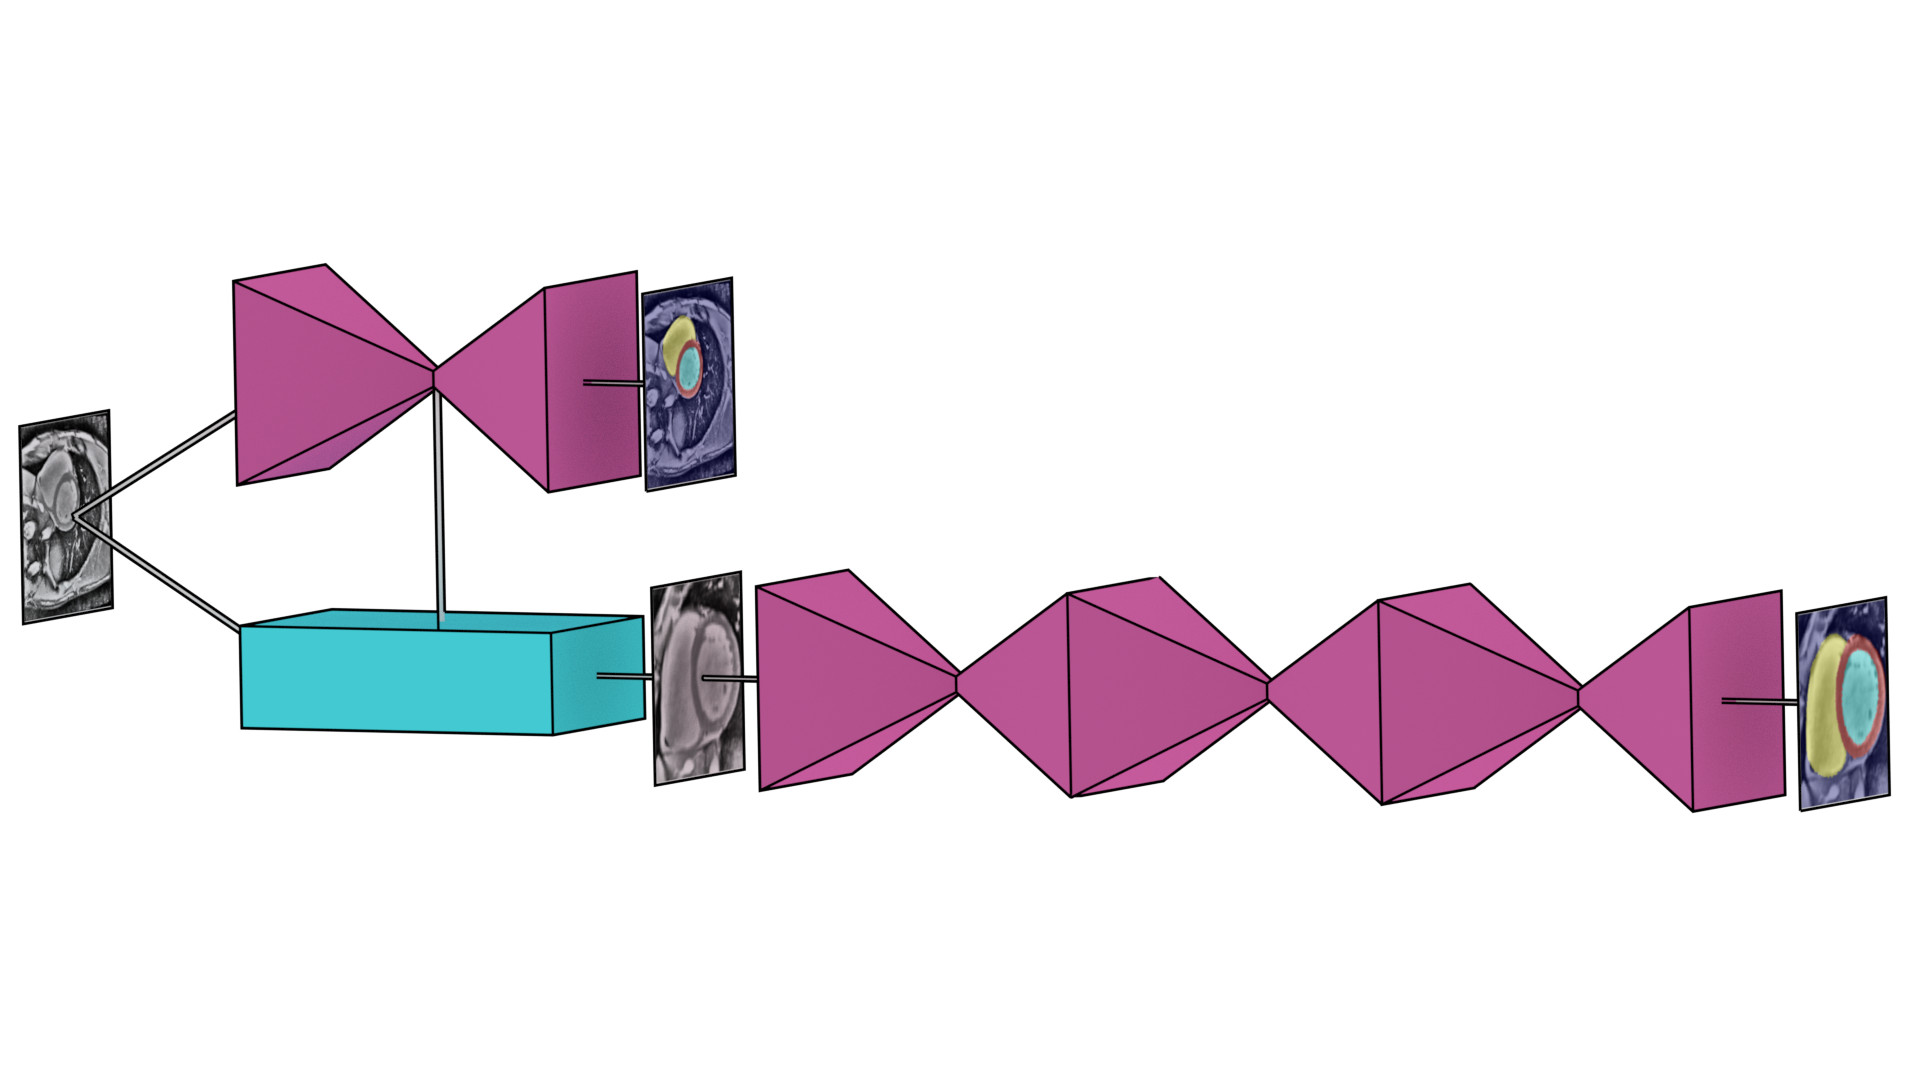
\includegraphics[clip, trim=0 260 0 260, width=1.0\textwidth]{./data/ohm-net-architecture.png}};

\node [anchor=south west] (a) at (0.025\tw,0.22\tw) {\large $\image$};
\node [anchor=south west] (b) at (0.35\tw,0.13\tw) {\large $\image^\prime$};
\node [anchor=south west] (c) at (0.35\tw,0.29\tw) {\large $S$};
\node [anchor=south west] (d) at (0.95\tw,0.13\tw) {\large $S^\prime$};
\node [anchor=south west] (e) at (0.17\tw,0.06\tw) {\large $\trans(\image, \tmat)$};

\draw [decorate,decoration={brace,amplitude=10pt},xshift=0pt,yshift=0pt](0.1275\tw,0.3\tw) -- (0.34\tw,0.3\tw) node [black,midway,xshift=0.0cm,yshift=+0.7cm] {(a) 粗分割模块};
\draw [decorate,decoration={brace,amplitude=10pt},xshift=0pt,yshift=0pt](0.3425\tw,0.045\tw) -- (0.1325\tw,0.045\tw) node [black,midway,xshift=0.0cm,yshift=-0.7cm] {(b) 变换模块};
\draw [decorate,decoration={brace,amplitude=10pt},xshift=0pt,yshift=0pt](0.4\tw,0.15\tw) -- (0.935\tw,0.15\tw) node [black,midway,xshift=0.0cm,yshift=+0.7cm] {(c) 细分割模块};
\end{tikzpicture}

\caption[\captiontitle]{\captiontitle{}.  (a) 将原始的 \SSFP{} 图像送入 \UNet{} 模块,得到一个粗分割输出 $S$.(b) 从该层 \UNet{} 中间(下采样)层输出的特征被用来给变换模块预测一个刚体仿射变换的参数 $\tmat$,该变换这可将输入图像变换到一个典型方向 $\image^\prime = \trans(\image, \tmat)$.(c) 这个变换后的图像就送入一个对堆叠的沙漏形网络对变换到典型方向的 $S^\prime$ 进行最后的细分割.需要说明的是,这里的所有模块都是从头开始端到端的训练的.}
\label{fig:omega-net-architecture}
\end{center}
\end{figure*}


二维静态图像序列(SSFP, steady state free precession)的左心和四腔心分割是进行容量估计(如射血分数,每搏量和心输出量);形态学特征(如心肌质地,壁厚等)和应力分析\citep{Peng2016}前的必要步骤.
然而,心脏的全自动分割依然是一个棘手的问题,主要是因为:

\begin{itemize}
\item 心脏大小、方向以及形态学上的生物差异.
\item 不同扫描仪器、流程和临床切面的对比度和外观差异.
\item 心内膜小梁和乳头肌的影响.
\item 心室心房之间以及心腔和血管之间的模糊边界
\end{itemize}

解决上述问题常用的有三种方法.
第一,对问题的范围进行限定,例如只对 SA 切面的左心肌和血池进行分割.
第二,增加用户交互,提供有效的初始化,额外的解剖标记或者错误修正.
第三,将心脏结构的先验知识融合到模型中.
显然,这些方法都不够理想:第一种方法限制了算法能够学习到的信息;第二种方法增加了医生的劳动;而第三种方法需要更加小心的设计算法. 

近来,深度神经网络(CNN)在自然图像分类 \citep{Krizhevsky2012,Simonyan2015} 和分割 \citep{Long2015,Noh2015,Yu2016} 以及生物医学图像分析 \citep{Ronneberger2015,Xie2015} 取得瞩目的成就.
已有研究将 CNN 分割应用到短轴切面 CMR 图像的左室血池(\citep{Tan2016,Poudel2016a,Tan2017},右室血池(\citep{Luo2016},以及同时对前述两者分割(\citep{Tran2016,Lieman-Sifry2017,Vigneault2017}).
这些方法要么定位和分割是分别进行\citep{Tan2016, Poudel2016a, Tan2017, Luo2016},要么是预先对图像进行裁剪,使得心脏就在图像中央,并占图像的主要部分,从而避开了定位任务\hl{\citep{Tran2016, Lieman-Sifry2017, Vigneault2017}}.他们都没有做端到端的定位和分割,也没有先变换到一个典型方向再做分割.

\renewcommand{\captiontitle}{典型方向下的临床切面}
\begin{figure*}
\begin{center}

\setlength{\tabcolsep}{1pt}

\begin{tabular}{ccccc}

\toprule
\SA{}(底层切片) & \SA{}(中间切片) & \SA{}(顶层切片) & \HLA{} & \VLA{} \\
\midrule

\multicolumn{5}{c}{未对齐方向的原始图像: $\image$} \\

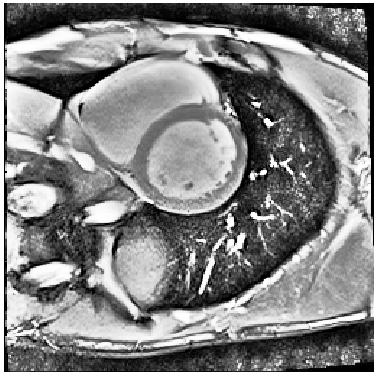
\includegraphics[width=0.19\textwidth]{./data/ohm/control/HCMNet_1100594/00_SAX/35_/im.png} &
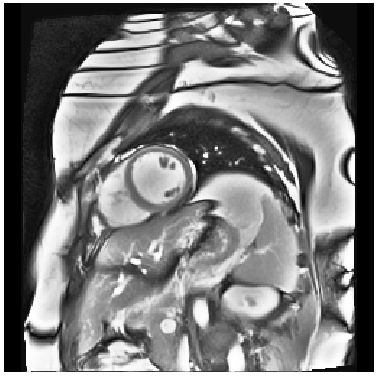
\includegraphics[width=0.19\textwidth]{./data/ohm/control/HCMNet_1100823/00_SAX/33_/im.png} &
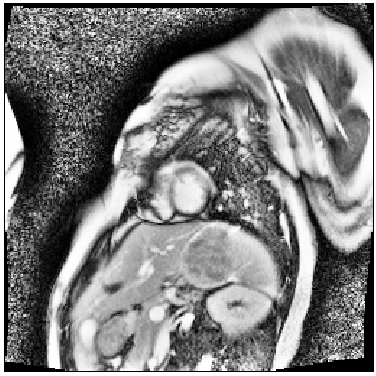
\includegraphics[width=0.19\textwidth]{./data/ohm/control/HCMNet_2600035/00_SAX/024_SA_CINE/im.png} &
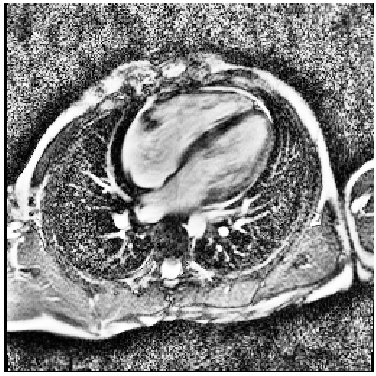
\includegraphics[width=0.19\textwidth]{./data/ohm/control/HCMNet_1700012/01_HLA/00/im.png} &
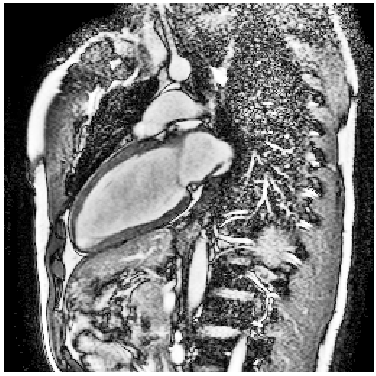
\includegraphics[width=0.19\textwidth]{./data/ohm/control/HCMNet_2100096/02_VLA/00/im.png} \\

\multicolumn{5}{c}{结构定位} \\

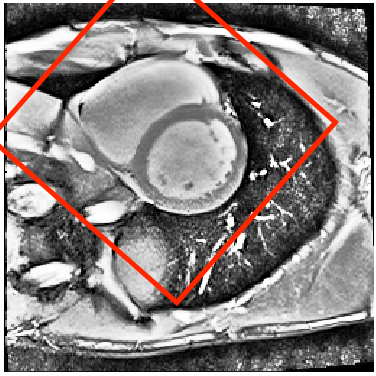
\includegraphics[width=0.19\textwidth]{./data/ohm/control/HCMNet_1100594/00_SAX/35_/im_det.png} &
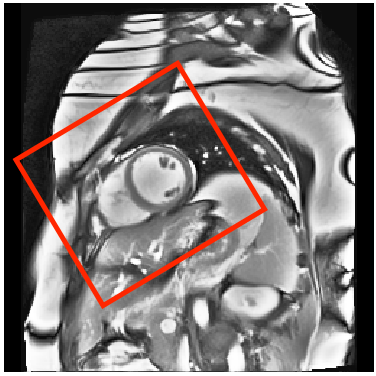
\includegraphics[width=0.19\textwidth]{./data/ohm/control/HCMNet_1100823/00_SAX/33_/im_det.png} &
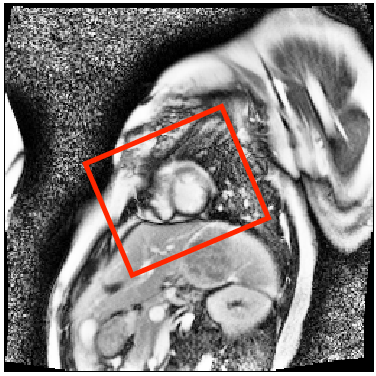
\includegraphics[width=0.19\textwidth]{./data/ohm/control/HCMNet_2600035/00_SAX/024_SA_CINE/im_det.png} &
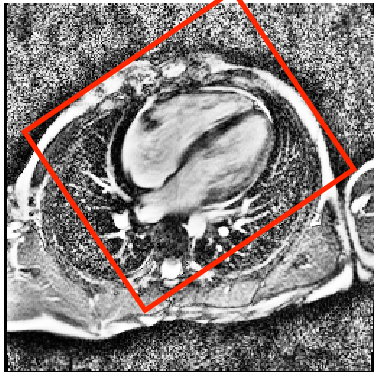
\includegraphics[width=0.19\textwidth]{./data/ohm/control/HCMNet_1700012/01_HLA/00/im_det.png} &
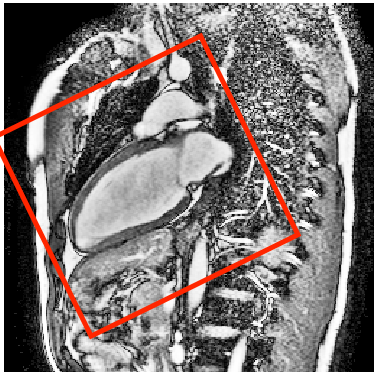
\includegraphics[width=0.19\textwidth]{./data/ohm/control/HCMNet_2100096/02_VLA/00/im_det.png} \\

\multicolumn{5}{c}{变换到典型方向的图像:$\image^\prime = \trans(\image,M)$} \\

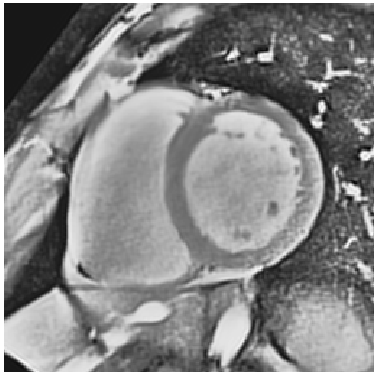
\includegraphics[width=0.19\textwidth]{./data/ohm/control/HCMNet_1100594/00_SAX/35_/im_t.png} &
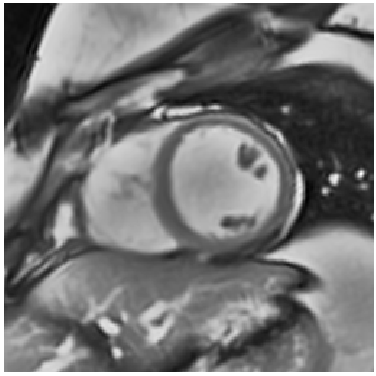
\includegraphics[width=0.19\textwidth]{./data/ohm/control/HCMNet_1100823/00_SAX/33_/im_t.png} &
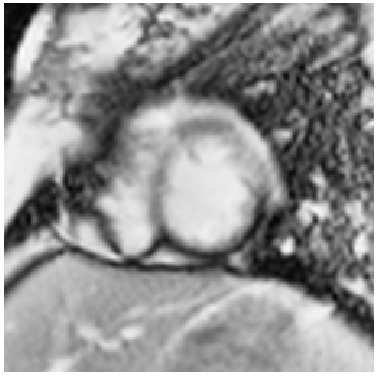
\includegraphics[width=0.19\textwidth]{./data/ohm/control/HCMNet_2600035/00_SAX/024_SA_CINE/im_t.png} &
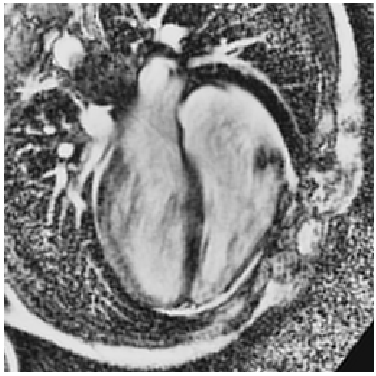
\includegraphics[width=0.19\textwidth]{./data/ohm/control/HCMNet_1700012/01_HLA/00/im_t.png} &
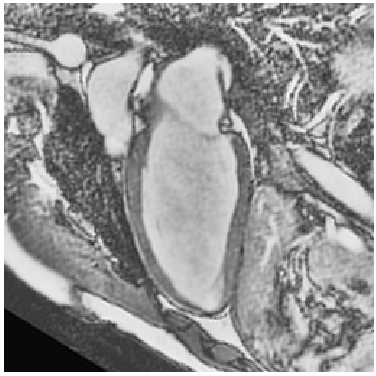
\includegraphics[width=0.19\textwidth]{./data/ohm/control/HCMNet_2100096/02_VLA/00/im_t.png} \\
\bottomrule

\end{tabular}

\caption[\captiontitle]{\captiontitle{}.
图中上面一行为短轴面(\SA{})、四腔切面(\HLA{})和两腔(\VLA{})的图像,下面一行为对应的经过一个刚体、仿射变换后变换到一个典型方向的图像.
按照临床习惯,心脏已经经过了旋转,使得 \SA{} 面的右室在放射学上的图像右侧,而左室在 \HLA{} 和 \VLA{} 面的方向是沿着长轴方向的.
心脏区域也已经移中并缩放,占到图像大小的 $90\%$.
请注意未经过方向对齐的图像中心脏的大小、方向和外观的异质,这大大增加了分割的难度.
}
\label{fig:canonical-orientation}
\end{center}
\end{figure*}


\hl{
在深度学习领域,CNN 网络的不变性仅仅是来自平均化池化和最大化池化的组合.
然而,卷积或者相关操作有几个缺陷:它既不是旋转不变或等变的,也不是尺度不变的,因此需要需要大量的数据来表示这些可能的变化 \citep{Sifre2013, Dieleman2015}.
}
在本文中,我们提出 \omeganet{}(Omega-Net),一个全新的 CNN 网络架构,来解决这三个问题(图 \ref{fig:omega-net-architecture}).

简单起见,尽管更加复杂的网络,例如 ResNet \citep{He2016} 也可以使用,我们还是使用 \UNet{} 作为粗分割和细分割的组成模块 \citep{Ronneberger2015}.
受空间变换网络 \citep{Jaderberg2015} 的启发,我们设计了一个完全不同的网络来实现定位和变换到一个典型方向的功能.

变换后的图像被送入一个由沙漏形网络堆叠而成的细分割网络 \citep{Newell2016}.
\hl{
在这样一个堆叠的沙漏形网络中,多个 \UNet{} 模块完成分割,并将输出传到下一个 \UNet{} 中.
这样的结构已经被证明可以逐渐降低误差,提升准确率 \citep{Newell2016}.
}

我们展示了 \omeganet{} 可以进行全自动的分割出三个标准切面(SA,短轴面;4C,四腔心面;2C,两腔心面)中的五个前景类别(左室心肌,左右心房和左右心室),参见图 \ref{fig:canonical-orientation}.
而且,我们的网络在多中心点的患者上测试,这些患者患有肥厚性心肌病(\HCM{}).这大大增加了问题的难度与复杂性,因为左室的巨大差异.
网络性能,以 \IoU{} 计算,比起没有使用定位和方向变换的 \UNet{} 分割结果有明显的提升($0.858$ vs $0.834$).
\hl{
此外,我们在 2017 MICCAI 自动心脏病诊断挑战公开数据集上(\miccaidata{}) dataset,\footnote{\url{https://www.creatis.insa-lyon.fr/Challenge/acdc/}}从头开始训练,并取得了比现有结果\citep{Isensee2018}更好的成绩,仅有左室心肌的分割略差.
}


%%%%%%%%%%%%%%%%%%%%%%%%%%%%%%%%%%%%%%%%%%%%%%%%%%%%%%%%%%%%%%%%%%%%%%%%%%%%%%%%
%% Methods
%%%%%%%%%%%%%%%%%%%%%%%%%%%%%%%%%%%%%%%%%%%%%%%%%%%%%%%%%%%%%%%%%%%%%%%%%%%%%%%%

\section{方法} \label{methods}


\hl{
由于 CNN 缺少旋转不变性,现有的方法就只能使用大量的数据来进行训练,这样才能代表所有可能出现的情况(例如旋转,裁剪等等).
我们推测,对于生物医学图像来说,如果我们先将感兴趣的结构检测处理,然后变换到一个典型方向,则可以更加高效地进行分割.
}
所谓的典型方向(\CMR{})是针对不同的标准切面进行定义的(图 \ref{fig:canonical-orientation}).
我们提出的心脏 \SSFP{} 图像分割网络是端到端训练的,而且允许定位、对齐和分割任务互相影响促进.
我们的模型由三个阶段组成.
第一,将全尺寸的原始图像 $\image$ 输入到一个 \UNet{} 模块 \S \ref{sec:unet} 进行粗分割. 
第二,利用 \UNet{} 中间(下采样)的特征来预测一个刚体仿射变换矩阵 $\tmat$,将图像变换到一个典型方向 $\timage = \trans(\image, \tmat)$ (\S\ref{sec:stn}).
第三,用一个堆叠的沙漏形模块(\S\ref{sec:hourglass})对变换后的图像 $\timage$ 进行分割.
以下小节将对每个模块进行详细的讨论.
为了方便,我们在字母上加个小帽表示真实值(如 $\hat{x}$),在字母上加一撇表示预测值(如 $x^\prime$).

\subsection{粗分割 (\UNet{}) 模块}\label{sec:unet}

\renewcommand{\captiontitle}{\UNet{} 模块}
\begin{figure}
\centering
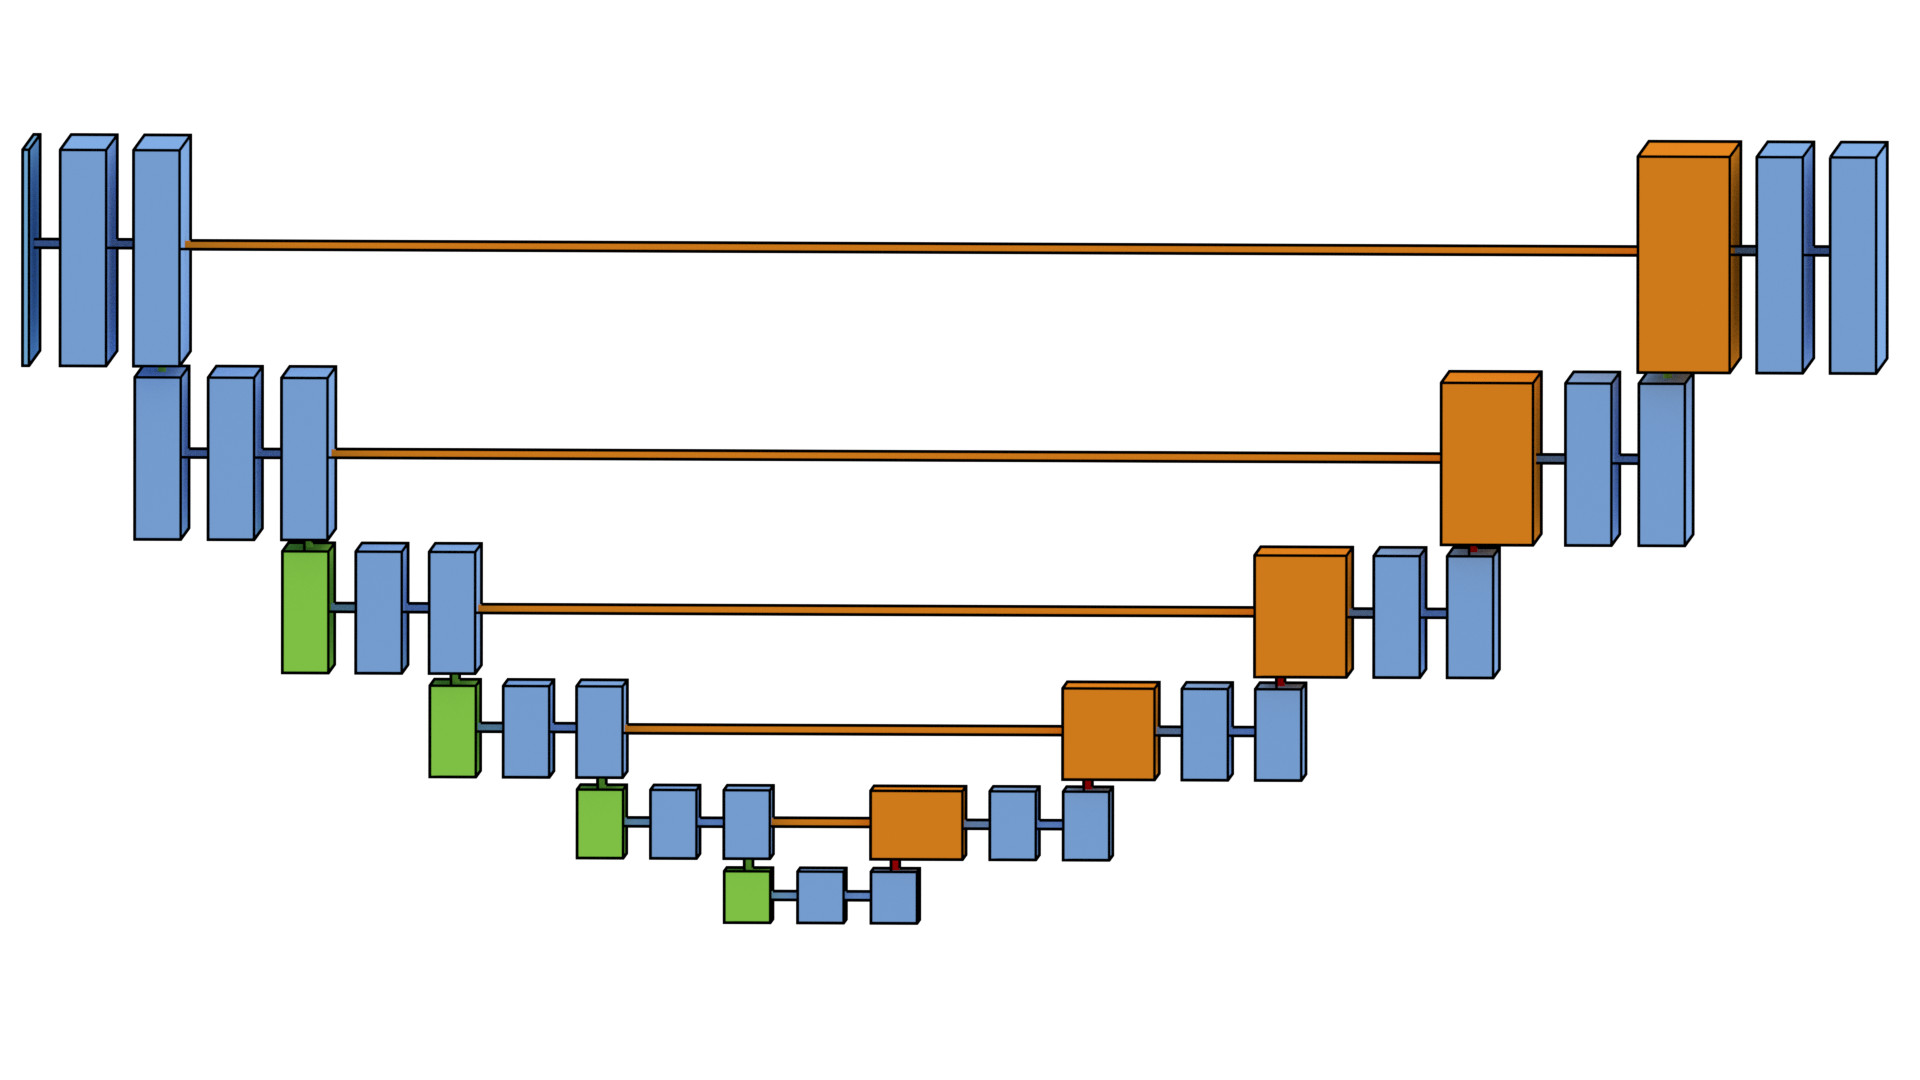
\includegraphics[clip, trim=0 0 0 0,width=0.5\textwidth]{./data/unet-module.png}
\caption[\captiontitle]{\captiontitle{}.  输入图像尺寸为 $\N \times \N \times N$,其中 $N$ 通道数(所有网络的通道数均为 $1$).
蓝色、绿色和橙色方框对应着多通道的特征图.绿色对应的是下采样的特征图,橙色对应的是将结果与特征图的拼接.}
\label{fig:unet-module}
\end{figure}



本文提出的网络使用了一个在生物医学图像分割任务\citep{Long2015,Ronneberger2015,Xie2015}中表现优异的深度卷积神经网络 \UNet{} 模块(图 \ref{fig:unet-module}).
\UNet{} 模块由左侧的下采样和右侧的上采样组成.
下采样部分由一个典型的 CNN 网络 \citep{Krizhevsky2012,Simonyan2015} 组成,两个 $3 \times 3$ 的卷积层,一个 \ReLU{} 激活层,一个 $2 \times 2$ 的最大化池化层,这些层不断重复堆叠,应用到输入图像和特征图.
下采样部分,经过不断的 $2 \times 2$ 上采样,\ReLU{} 激活和 $3 \times 3$ 卷积,下采样的图像恢复到原来的尺寸.
为了提供更加准确的分割边界,我们使用了跳跃连接,使得相同层级的下采样和下采样的输出串联到一起.
批标准化 \mbox{\citep{Ioffe2015}} 已经被证明可以有效地避免梯度消失现象,所以我们在每一个卷积层与激活层之间均加入了批标准化操作.
\UNet{} 模块的损失函数 $L_{S_U}$ 为交叉熵损失函数,也就是输出 $P$ 与真实值 $\hat{S}$ 的交叉熵,

\begin{equation}\label{eqn:unet-loss}
L_{S_U} = -\frac{1}{HW} \sum_{\forall h,w} \CCE(P_{h,w}, \hat{S}_{h,w}),
\end{equation}

\noindent 其中

\begin{equation}\label{eqn:cross-entropy}
\CCE(x, \hat{x}) = - \hat{x} \log(x) + (1 - \hat{x}) \log(1 - x).
\end{equation}

\hl{
$H$ 和 $W$ 分别为输入图像的高度和宽度,$h$ 和 $w$ 为对应的索引.
}

\subsection{\hl{变换} 模块}\label{sec:stn}

\renewcommand{\captiontitle}{空间变换网络模块}
\begin{figure}
\begin{center}

\begin{tikzpicture}
\node [anchor=south west] (image) at (0,0) {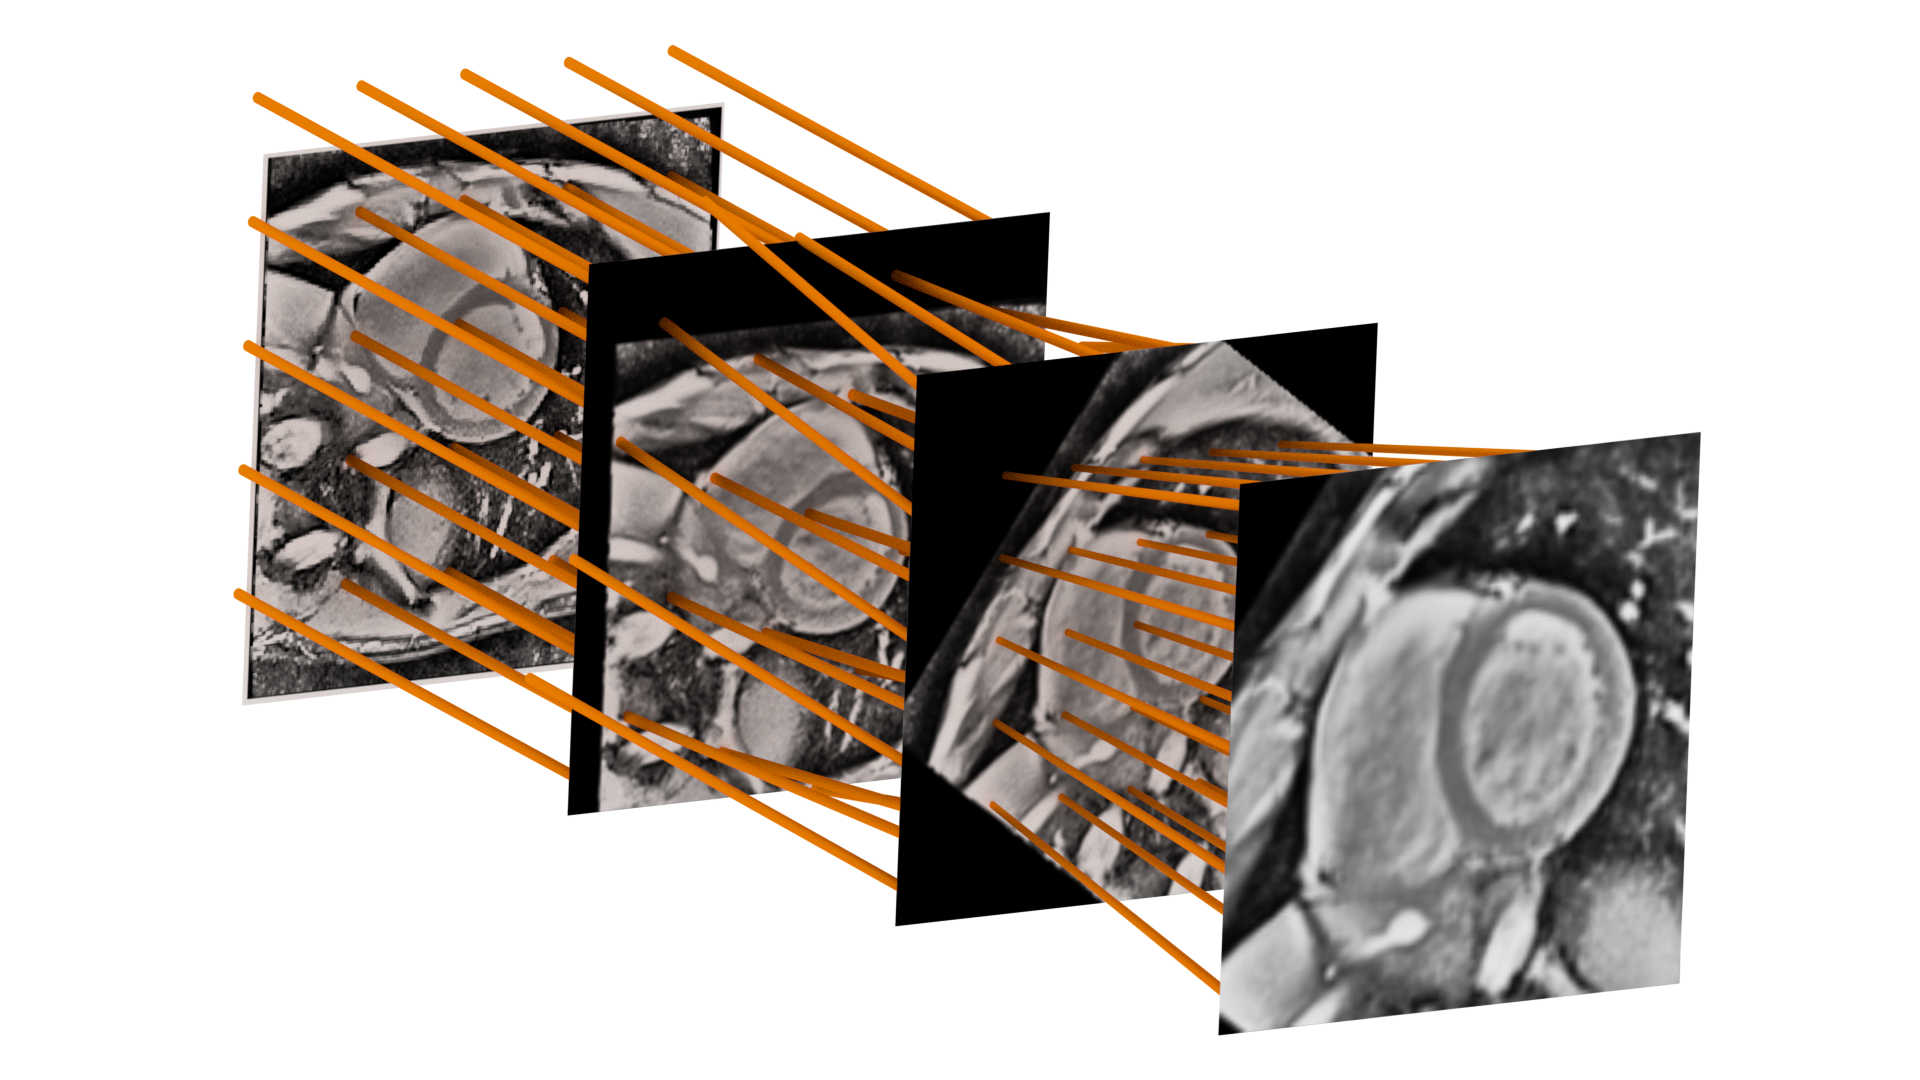
\includegraphics[width=0.5\textwidth]{./data/sampler.png}};
\draw [decorate,decoration={brace,amplitude=10pt},xshift=0pt,yshift=0pt](2.8,1.317) -- (1.25,1.85) node [black,midway,xshift=-0.3cm,yshift=-0.7cm] {\footnotesize $\image_2 = \trans(\image, T)$};
\draw [decorate,decoration={brace,amplitude=10pt},xshift=0pt,yshift=0pt](4.35,0.783) -- (2.8,1.317) node [black,midway,xshift=-0.3cm,yshift=-0.7cm] {\footnotesize $\image_3 = \trans(\image_2, R)$};
\draw [decorate,decoration={brace,amplitude=10pt},xshift=0pt,yshift=0pt](5.9,0.25) -- (4.35,0.783) node [black,midway,xshift=-0.3cm,yshift=-0.7cm] {\footnotesize $\trans(\image_3, S)$};
\end{tikzpicture}

\caption[\captiontitle]{\captiontitle{}.请注意,在实际的实现中,所有的变换都是相对于输入图像 $\image$ (即 $\trans(\image, T)$,$\trans(\image, RT)$和$\trans(\image, SRT)$)的变换;我们在此处只是为了清晰地说明这是连续处理的步骤.}
\label{fig:stn-module}
\end{center}
\end{figure}



空间变换网络(\STN{}) 最初是作为分类任务的通用层提出的,目的是提升空间不变性\citep{Jaderberg2015}.
\STN{} 模块本身由三个子模块组成:一个定位模块(\LocNet{})模块,用于预测一个刚体仿射变换矩阵 $\tmat$;一个网格生成器,用于实现变换 $\trans$;一个采样器,用于实现插值.

在文献 \citep{Jaderberg2015} 中,\STN{} 网络可以学习到适合分类任务的最佳变换参数;而且也不需要给出真实值,预测的变换矩阵用于将中间层的\emph{特征图}进行变换.
但是,在本文的应用中,我们感兴趣的是学习如何将\emph{输入图像}变换到一个标准的临床方向,从而指引语义分割任务.

%%%%%%%%%%%%%%%%%%%%%%%%%%%%%%%%%%%%%%%%%%
% 	Locnet
%%%%%%%%%%%%%%%%%%%%%%%%%%%%%%%%%%%%%%%%%%
\subsubsection{定位网络(\LocNet{})}

给出一个心脏分割图像,一个人类专家可以从直觉上给出平移、旋转和缩放信息.
基于这一假设,我们从 \UNet{} 的最后一个最大化池化层的输出引出一个小小的定位网络(\LocNet{})分支,从而预测变换参数(图 \ref{fig:stn-module}).
我们将变换限定为平移、旋转和缩放,则仿射变换矩阵可以分解为三个矩阵:

$$
\tmat = SRT,
$$

\noindent 其中 $T$ 为平移变换矩阵:

$$
T =
\begin{bmatrix}
1 & 0 & t_x \\
0 & 1 & t_y \\
0 & 0 & 1 \\
\end{bmatrix};
$$

\noindent $R$ 为旋转变换矩阵(逆时针):

$$
R =
\begin{bmatrix}
\cos(\theta) & - \sin(\theta) & 0 \\
\sin(\theta) & \cos(\theta) & 0 \\
0 & 0 & 1 \\
\end{bmatrix};
$$

\noindent 以及 $S$ 为缩放变换矩阵:

$$
S =
\begin{bmatrix}
s & 0 & 0 \\
0 & s & 0 \\
0 & 0 & 1 \\
\end{bmatrix}.
$$

\noindent 图像定义在一个归一化的坐标空间 $\{x, y\} \in [-1, +1]$,这样它的旋转是相对于图像中心点来说的.

定位网络 \LocNet{} 只需要学习和预测相关的参数 $\tparams = \begin{bmatrix}t_x & t_y & \theta & s \end{bmatrix}^\top$.
我们在训练中提供真实值 $\hat{\tparams} = \begin{bmatrix} \hat{t_x} & \hat{t_y} & \hat{\theta} & \hat{s} \end{bmatrix}$,并不断地最小化两个损失,即 \emph{矩阵损失(matrix losses)}和\emph{图像损失(image losses)}.

矩阵损失为真实值与预测值 $L_{t_x}$, $L_{t_y}$, $L_\theta$, $L_s$ 之间的回归损失.
对于缩放和平移来说,我们使用了均方根误差(\MSE{})作为损失函数:

\begin{align}
L_{t_x} & = \frac{1}{2} (t_x - \hat{t_x})^2, \label{eqn:attn-mat-loss-tx} \\
L_{t_y} & = \frac{1}{2} (t_y - \hat{t_y})^2, \mathrm{~and} \label{eqn:attn-mat-loss-ty} \\
L_s     & = \frac{1}{2} (s - \hat{s})^2. \label{eqn:attn-mat-loss-s}
\end{align}

\renewcommand{\captiontitle}{均方根误差(\MSE{}) vs 包裹的均方根误差(\MSWE{})}
\begin{figure*}
\begin{center}
\begin{subfigure}{0.48\textwidth}
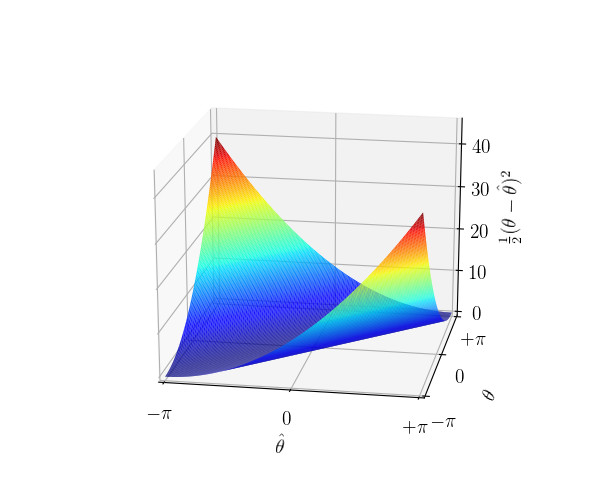
\includegraphics[clip, trim=90 30 50 70,width=1.0\textwidth]{./data/phase-loss.png}
\caption{均方根误差(\MSE{})}
\end{subfigure}
\begin{subfigure}{0.48\textwidth}
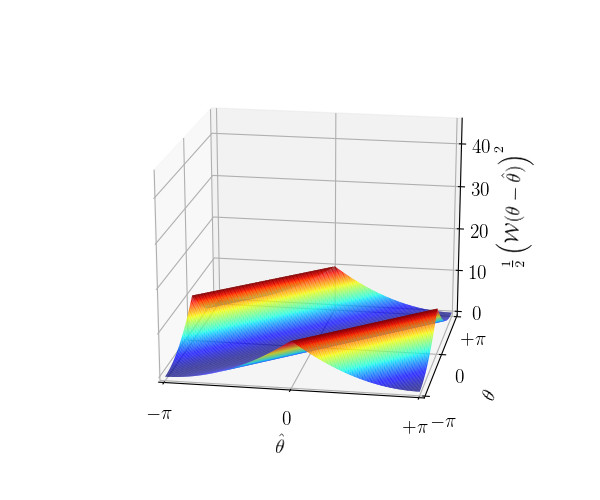
\includegraphics[clip, trim=90 30 50 70,width=1.0\textwidth]{./data/wrapped-phase-loss.png}
\caption{包裹的均方根误差(\MSWE{})}
\end{subfigure}
\caption[\captiontitle]{\captiontitle{}.}
\label{fig:wrapped-phase-loss}
\end{center}
\end{figure*}



由于周期性,简单的 \MSE{} 并不适合作为参数 $\theta$ 的损失函数.举例来说,当预测值为 $\theta = -\pi$,真实值为 $\hat{\theta} = \pi$ 的时候,\MSE{} 的损失值也最大.
因此,我们提出一个包裹的 \MSE{} 损失函数(\MSWE{}),如图 \ref{fig:wrapped-phase-loss} 所示,我们将 $\theta - \hat{\theta}$ 包裹起来,使其取值范围为 $[-\pi, \pi)$,然后再用标准的 \MSE{} 计算,

\begin{equation}
L_\theta = \frac{1}{2} \left(\wrap(\theta - \hat{\theta})\right)^2, \label{eqn:attn-mat-loss-r}
\end{equation}

\noindent 其中这个包裹的操作 $\wrap$ 定义为

$$
\wrap(\cdot) = \mod(\cdot + \pi, 2\pi) - \pi.
$$

仅仅基于这些损失进行变换模块的训练很容易导致过拟合.
为此,我们基于 \MSE{} 额外添加了变换后的图像的真实值$\hat{\tparams}$与预测值$\tparams$之间的正则化约束项:

\begin{align}
L_{\image_t}      & = \frac{1}{2} (\trans(\image, T  ) - \trans(\image, \hat{T}  ))^2,                     \label{eqn:attn-image-loss-t} \\
L_{\image_\theta} & = \frac{1}{2} (\trans(\image, RT ) - \trans(\image, \hat{R}\hat{T} ))^2, \mathrm{~and} \label{eqn:attn-image-loss-r} \\
L_{\image_s}      & = \frac{1}{2} (\trans(\image, SRT) - \trans(\image, \hat{S}\hat{R}\hat{T}))^2.         \label{eqn:attn-image-loss-s}
\end{align}

%%%%%%%%%%%%%%%%%%%%%%%%%%%%%%%%%%%%%%%%%%
% 	Sampler
%%%%%%%%%%%%%%%%%%%%%%%%%%%%%%%%%%%%%%%%%%
\subsubsection{网格生成和采样}

一般来说,一个 \ND{2} 网格生成器均匀采样 $G \in \Real^{2 \times H' \times W'}$,然后根据 \LocNet{} 预测的参数对他们进行变换.
在我们的应用中,我们生成三个这样的网格,每个的维度等于输入($H' = W' = \N$),并均匀延伸到图像大小($x \in [-1,1]$, $y \in [-1, 1]$).
随后,我们用 \LocNet{} 预测的参数$T$,$RT$和$SRT$将这些网格进行变换,从而确定原始图像中的哪些点需要采样.

采样器的输入参数为输入图像 $\image \in \Real^{H \times W \times C}$ 和变换网格 $G^\prime$,输出为一个重采样的图像 $\timage \in \Real^{H' \times W' \times C}$.
\footnote{\hl{为了完整性,我们引入了通道参数 $C$;然而,应该强调的是,我们的应用中输入为灰度图 $\image$,也就是 $C = 1$ 的情况.}}
对于每一个通道 $c \in [1 \twodots C ]$,$(h',w')$ 处的输出 $\timage_{h',w',c}$ 为输入值 $\image_{h,w,c}$ 在邻域 $G^\prime_{1,h',w'}, G^\prime_{2,h',w'}$ 的加权和,

\begin{align*}
\timage_{h',w',c} & = \sum^H_{h=1}\sum^W_{w=1}\image_{h, w, c} \\
                  & \cdot \max\left(0, 1-|\alpha_v G^\prime_{1, h', w'} + \beta_v - h| \right) \\
                  & \cdot \max\left(0, 1-|\alpha_u G^\prime_{2, h', w'} + \beta_u - w| \right),
\end{align*}

\noindent 其中

$$
\begin{aligned}
\alpha_v & = +\frac{H-1}{2},               \\
\beta_v  & = -\frac{H+1}{2},              \\
\alpha_u & = +\frac{W-1}{2}, \mathrm{ and} \\
\beta_u  & = - \frac{W+1}{2}.
\end{aligned}
$$

\noindent 这里的每一步计算都是可微的,这样就保证了模型可以端到端地进行训练.

%%%%%%%%%%%%%%%%%%%%%%%%%%%%%%%%%%%%%%%%%%
% 	Hourglass
%%%%%%%%%%%%%%%%%%%%%%%%%%%%%%%%%%%%%%%%%%
\subsection{细分割模块(堆叠的沙漏形网络)}\label{sec:hourglass}

变换模块的输出是已经变换到一个典型方向的了,接着就是送入一个堆叠的沙漏形网络结构中.
这个沙漏形网络由 $D = [1 \twodots 3]$ 个 \UNet{} 模块前后连接而成.每个 \UNet{} 模块产生一个分割输出 $S_{H,d}$,其中 $d \in [1 \twodots D]$.
第 $d$ 层的输出 $P^{H,d}_{h,w}$ 与真实值 $\hat{S}^\prime$ 的交叉熵可以按照公式 \eqref{eqn:cross-entropy} 进行计算,

\begin{equation}\label{eqn:hourglass-loss}
L_{S_{H,d}} = -\frac{1}{HW} \sum_{\forall h,w} \CCE(P^{H,d}_{h,w}\hat{S}^\prime_{h,w}).
\end{equation}

%%%%%%%%%%%%%%%%%%%%%%%%%%%%%%%%%%%%%%%%%%
% 	Summary
%%%%%%%%%%%%%%%%%%%%%%%%%%%%%%%%%%%%%%%%%%
\subsubsection{小结}

小结一下,我们使用损失函数 \cref{eqn:unet-loss} 来训练 \omeganet{} 的粗分割模块;四个矩阵损失函数 \cref{eqn:attn-image-loss-t,eqn:attn-image-loss-s,eqn:attn-image-loss-r} 来训练变换模块;以及一到三个损失函数 \cref{eqn:hourglass-loss} 来训练最后的细分割模块.
因此,总的损失函数就是:

\begin{equation}
\begin{aligned}
L_\Omega & = \alpha_1 L_{S_U} \\
  & + \alpha_2 (L_{t_x} + L_{t_y} + L_{\theta}+ L_{s}) \\
  & + \alpha_3 (L_{I_t} + L_{I_\theta} + L_{I_s}) \\
  & + \alpha_4 \sum_{d=1}^D L_{S_{H,d}}, \\
\end{aligned}
\end{equation}

\noindent 其中 $\alpha_1 = 100.0$,$\alpha_2 = 100.0$,$\alpha_3 = 0.1$,$\alpha_4 = 1.0$.
网络结构总结如表 \ref{tab:architecture-descriptions} 所示.

\hl{
尽管我们的输入数据经过了较小的刚体仿射变换进行数据增强,我们还要特别指出的是,细分割期间也进行了\emph{隐含的}数据增强,因为我们在粗分割的时候使用了变换网络.
}


%%%%%%%%%%%%%%%%%%%%%%%%%%%%%%%%%%%%%%%%%%%%%%%%%%%%%%%%%%%%%%%%%%%%%%%%%%%%%%%%
%% Experiments
%%%%%%%%%%%%%%%%%%%%%%%%%%%%%%%%%%%%%%%%%%%%%%%%%%%%%%%%%%%%%%%%%%%%%%%%%%%%%%%%

\section{实验} \label{experiments}


\subsection{\hl{HCMNet 数据集}}

\renewcommand{\captiontitle}{考虑中的 \CNN{} 网络结构变体}
\begin{table*}
\begin{center}
\begin{tabular}{lrrrrr} \hline
\toprule
名称      & \UNet{} 0 & \UNet{} 1 & \UNet{} 2 & \UNet{} 3 & 参数量(百万) \\
\midrule
网络 A & 128       & --        & --        & --        & \MillionsOfParamsA{} \\
网络 B & 64        & 64        & --        & --        & \MillionsOfParamsB{} \\
网络 C & 64        & 64        & 64        & --        & \MillionsOfParamsC{} \\
网络 D & 64        & 64        & 64        & 64        & \MillionsOfParamsD{} \\
\bottomrule
\end{tabular}
\caption[\captiontitle{}]{
\captiontitle{}.
\hl{
网络 A 是一个基线 \UNet{}(仅有粗分割模块,不含变换或者细分割模块).
网络 B、C 和 D 是细分割模块中分别有着 1、2和3个 \UNet{} 结构的完整的 \omeganet{} 网络结构.
表中还给出了每一个 \UNet{} 模块的特征向量长度.
}
}
\label{tab:architecture-descriptions}
\end{center}
\end{table*}


HCMNet 数据集包含 \NumPtT{} 个样本,其中 \NumPtO{} 个患有肥厚性心肌病,\NumPtC{} 为健康人 \citep{Ho2017}.
心脏核磁共振 \CMR{} 检查由十个临床中心于 2009 到 2011 年期间按照标准流程进行.
其中九个使用 1.5-T 核磁共振,一个使用 3-T 核磁共振.
我们采集了三个 \SA{} 切面,一个 \HLA{} 切面和一个 \VLA{} 切面的 \SSFP{} 序列.
\hl{
图像的平面间隔为 $\SpacingMU{} \pm \SpacingSD{}$mm,尺寸为 $\MatrixMU{} \pm \MatrixSD{}$ 像素;更加详细的信息可以参考文献 \citet{Ho2017} 的补充材料.
}

左室心肌和其他所有四个心腔都在 \SA{},\HLA{} 和 \VLA{} 切面进行手动分割标注(应当注意到,并不是所有的类别都可以在 \SA{} 和 \VLA{} 切面看到).
\hl{
\ND{2} 时间卷数据会送入 ITK-Snap \citep{Yushkevich2006} 中去;每隔五帧做一个手动的分割标注,而剩余的图像的标注由插值算法自动产生.(分割由本文第一作者完成,他有有着五年的手动分割标注 \CMR{} 的经验).
}
\LV{} 和 \RV{} 切面的心肌不包含乳头肌和小梁.

每一卷数据数据都被适当地裁剪或者补零到 $\N \times \N$ 的空间尺寸,而时间轴的范围为 $\NumFramesMin{}$ 到 $\NumFramesMax{}$ 帧.
不均匀的背景光照均做了修正,然后进行直方图均衡处理.
每一个单独的图像都做了归一化处理,也就是减去均值再除以标准差,然后在送入 \CNN{} 网络.

\subsubsection{训练与交叉验证}

至于交叉验证,所有的被试分成了三份($\NumImFoldA{}$,$\NumImFoldB{}$,$\NumImFoldC{}$ 张图),并确保属于一个被试者的图像都分到了同一组中.
每一个网络(见表 \ref{tab:architecture-descriptions})都在其中两组中训练,然后在剩下那组进行测试,且包括所有的组合.
\hl{
网络 A 仅有粗分割模块;考虑到 \UNet{} 在生物医学图像分割任务中表现不错,这就是个基线水平.
网络 B、C 和 D 分别为细分割模块使用 1、2 和 3 个 \UNet{} 模块的 \omeganet{} 网络.
}

网络使用正交化的权重 \hl{\citep{Saxe2013}} 初始化,并使用 Adam 优化器 \citep{Kingma2015} 优化.
学习率初始化为 $0.001$,并每隔 $26$ 代衰减为原来的 $0.1$.
为了避免过拟合,我们使用数据增强(平移和缩放 $\pm \AugTrans{}\%$;旋转 $\pm \AugRot{}$\degree),并设置粗分割模块的权重衰减系数为 $\weightdecay{}$.
值得注意的是,数据增强也\emph{隐含}在最后的细分割模块,因为前面用了变换网络.我们还对每一时间序列做了单独的数据增强.

\subsubsection{性能评价指标}

我们计算每一图像的预测值与真实值之间的加权的 \IoU{} 来衡量网络性能.
对于二值图像(只有一个前景和一个背景)来说,真实值 $I_T$ 和预测值 $I_P$ 的 \IoU{}(也称 Jaccard 系数)定义为:

\begin{equation}
\IoU{} \left( I_T, I_P \right) = \frac{|I_T \cap I_P|}{|I_T \cup I_P|},
\end{equation}

\noindent 注意,在代码实现中应给分母加上一个较小的数字,以避免除以零的情况.
为了将 \IoU{} 扩展到多类的情况,我们先分别计算每一类与背景的 \IoU{}.
然后计算一个加权的 \IoU{},其中的权值由这些类别占所有类别的比重决定,也就是求出了一个加权的均值前景 \IoU{}.

\subsubsection{实现}

这个模型使用 Tensorflow \hl{\citep{Chollet2015,Abadi2016}} 的 Keras 接口,用 Python 语言实现,并使用一块 12 GB 显存的英伟达 Titan X 图形处理器(GPU)训练.
所有的网络在训练中都需要大约 20 分钟迭代一次.
而在测试阶段,网络预测出分割结果的速度大约在 15 帧每秒.

\hl{
\subsection{2017 MICCAI \miccaidata{} 数据集}

网络 B 从头开始在 2017 MICCAI \miccaidata{} 数据集上训练.
训练数据包含 100 个患者(20 个正常,20 个心肌梗塞,20 个扩张型心肌病 20 个肥厚性心肌病和 20 个右室心脏病)的 \SA{} 切面数据.

所有切片的数据都提供了舒张末期和收缩末期左室心肌,左室血池和右室血池的真实分割标签
为了能与 \miccaidata{} 的结果进行对比,网络的性能评估同时使用了 \IoU{} 和 Dice 系数:

\begin{equation}
\mathrm{Dice} \left( I_T, I_P \right) = \frac{2|I_T \cap I_P|}{|I_T| + |I_P|},
\end{equation}

\noindent 根据目前最优的结果 \citep{Isensee2017,Isensee2018},网络使用了五折交叉验证来训练.
}


%%%%%%%%%%%%%%%%%%%%%%%%%%%%%%%%%%%%%%%%%%%%%%%%%%%%%%%%%%%%%%%%%%%%%%%%%%%%%%%%
%% Results
%%%%%%%%%%%%%%%%%%%%%%%%%%%%%%%%%%%%%%%%%%%%%%%%%%%%%%%%%%%%%%%%%%%%%%%%%%%%%%%%

\section{结果} \label{results}

\subsection{\hl{HCMNet 数据集}}

% {A,B,C,D}{S,H,V}{M,H,L}{Ze,On,Tw,Th}
% {Network}{View}{Quartile}{Hourglass}
\renewcommand{\captiontitle}{网络性能评估}
\begin{sidewaystable*}
\begin{center}
\begin{tabular}{ccccccc} \hline
\toprule
名称      & View   & \UNet{} 0                 & \UNet{} 1                 & \UNet{} 2                 & \UNet{} 3                 \\
\midrule
网络 A & All    & $\AAMZe~[\AALZe,~\AAHZe]$ & --                        & --                        & --                        \\
          & \SA{}  & $\ASMZe~[\ASLZe,~\ASHZe]$ & --                        & --                        & --                        \\
          & \HLA{} & $\AHMZe~[\AHLZe,~\AHHZe]$ & --                        & --                        & --                        \\
          & \VLA{} & $\AVMZe~[\AVLZe,~\AVHZe]$ & --                        & --                        & --                        \\
\midrule
网络 B & All    & $\BAMZe~[\BALZe,~\BAHZe]$ & $\BAMOn~[\BALOn,~\BAHOn]$ & --                        & --                        \\
          & \SA{}  & $\BSMZe~[\BSLZe,~\BSHZe]$ & $\BSMOn~[\BSLOn,~\BSHOn]$ & --                        & --                        \\
          & \HLA{} & $\BHMZe~[\BHLZe,~\BHHZe]$ & $\BHMOn~[\BHLOn,~\BHHOn]$ & --                        & --                        \\
          & \VLA{} & $\BVMZe~[\BVLZe,~\BVHZe]$ & $\BVMOn~[\BVLOn,~\BVHOn]$ & --                        & --                        \\
\midrule
网络 C & All    & $\CAMZe~[\CALZe,~\CAHZe]$ & $\CAMOn~[\CALOn,~\CAHOn]$ & $\CAMTw~[\CALTw,~\CAHTw]$ & --                        \\
          & \SA{}  & $\CSMZe~[\CSLZe,~\CSHZe]$ & $\CSMOn~[\CSLOn,~\CSHOn]$ & $\CSMTw~[\CSLTw,~\CSHTw]$ & --                        \\
          & \HLA{} & $\CHMZe~[\CHLZe,~\CHHZe]$ & $\CHMOn~[\CHLOn,~\CHHOn]$ & $\CHMTw~[\CHLTw,~\CHHTw]$ & --                        \\
          & \VLA{} & $\CVMZe~[\CVLZe,~\CVHZe]$ & $\CVMOn~[\CVLOn,~\CVHOn]$ & $\CVMTw~[\CVLTw,~\CVHTw]$ & --                        \\
\midrule
网络 D & All    & $\DAMZe~[\DALZe,~\DAHZe]$ & $\DAMOn~[\DALOn,~\DAHOn]$ & $\DAMTw~[\DALTw,~\DAHTw]$ & $\DAMTh~[\DALTh,~\DAHTh]$ \\
          & \SA{}  & $\DSMZe~[\DSLZe,~\DSHZe]$ & $\DSMOn~[\DSLOn,~\DSHOn]$ & $\DSMTw~[\DSLTw,~\DSHTw]$ & $\DSMTh~[\DSLTh,~\DSHTh]$ \\
          & \HLA{} & $\DHMZe~[\DHLZe,~\DHHZe]$ & $\DHMOn~[\DHLOn,~\DHHOn]$ & $\DHMTw~[\DHLTw,~\DHHTw]$ & $\DHMTh~[\DHLTh,~\DHHTh]$ \\
          & \VLA{} & $\DVMZe~[\DVLZe,~\DVHZe]$ & $\DVMOn~[\DVLOn,~\DVHOn]$ & $\DVMTw~[\DVLTw,~\DVHTw]$ & $\DVMTh~[\DVLTh,~\DVHTh]$ \\
\bottomrule
\end{tabular}
\caption[\captiontitle{}]{\captiontitle{}.
\hl{
表中列出了所有的切面以及所有网络的加权的前景 \IoU{},并给出了四分位数范围的中值.
}
\SA{} 切面的网络性能变现最佳,\HLA{} 切面最差,但是他们的差异并不大.
}
\label{tab:architectureaccuracy}
\end{center}
\end{sidewaystable*}


\subsubsection{\hl{分割}}

我们分别计算了每一幅图的加权的前景 \IoU{},并给出所有预测值的中值和 \IQR{} 值.
详细的结果可以参见表 \ref{tab:architectureaccuracy}.

\renewcommand{\captiontitle}{各个网络加权的前景 \IoU{} 和网络深度关系}
\begin{figure}
\begin{center}
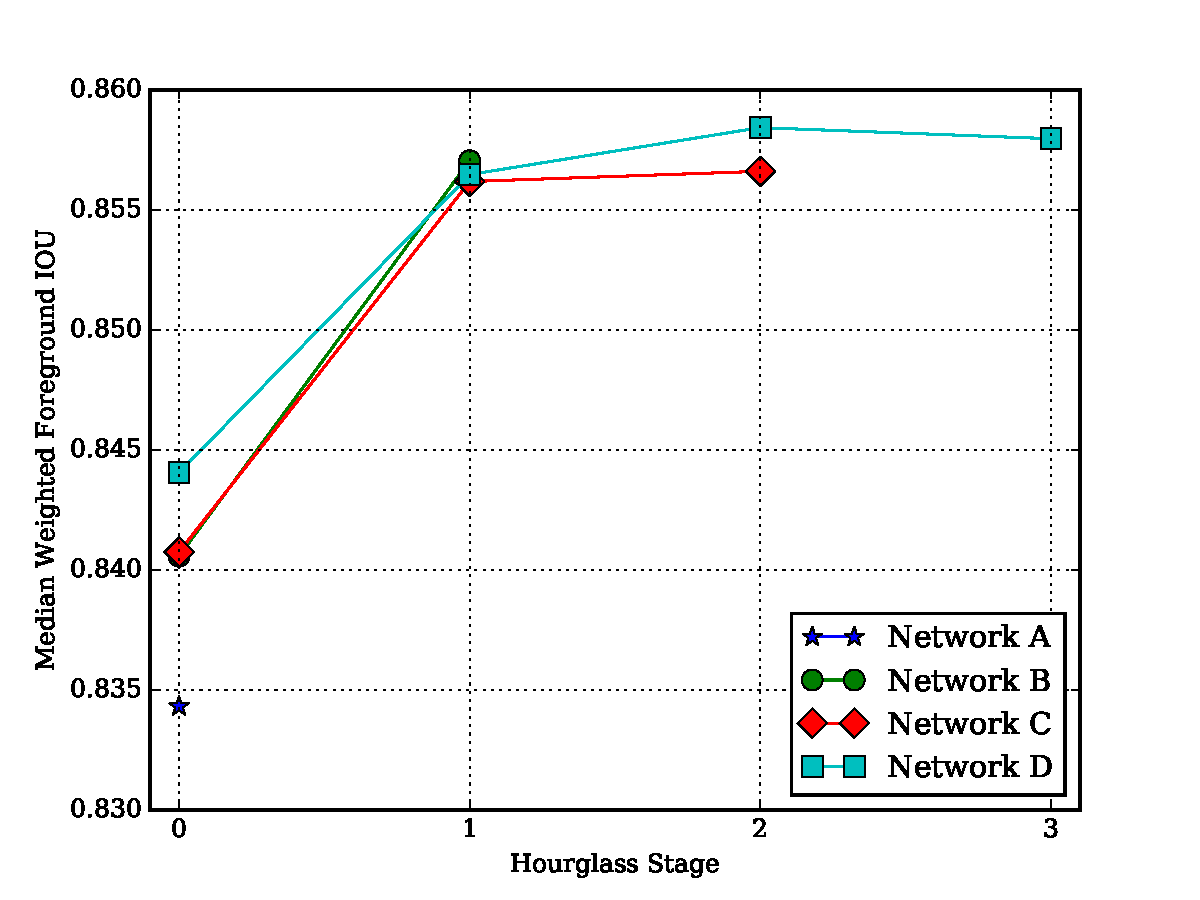
\includegraphics[width=0.5\textwidth]{./data/trendline.pdf}
\caption[\captiontitle]{\captiontitle{}.}
\label{fig:hourglass-accuracy}
\end{center}
\end{figure}


我们对每一个 \UNet{} 中间层的性能也进行了评估,详细内容见图 \ref{fig:hourglass-accuracy}.

\begin{itemize}
\item 虽然网络 A 的参数量最多,但是添加细分割模块可以在粗分割的基础上有效的提升网络性能;
即,网络 B 和 C 的粗分割模块的性能提升了 $\approx~0.007$,网络 D 的粗分割模块也比网络 B 和 C 性能提升了 $\approx~0.003$.
\item 粗分割和细分割之间也有明显的性能提升,即 \UNet{}s 0 和 1(网络 B、C 和 D 分别提升了 $\approx~0.016$,$\approx~0.015$ 和 $\approx~0.012$).
\item 在网络 C 和 D 中,没有观察到细分割模块中前后的 \UNet{}s 有显著的性能提升.
\end{itemize}

\renewcommand{\captiontitle}{每一切面和类别的 \IoU{} 直方图}
\begin{figure*}
\begin{center}
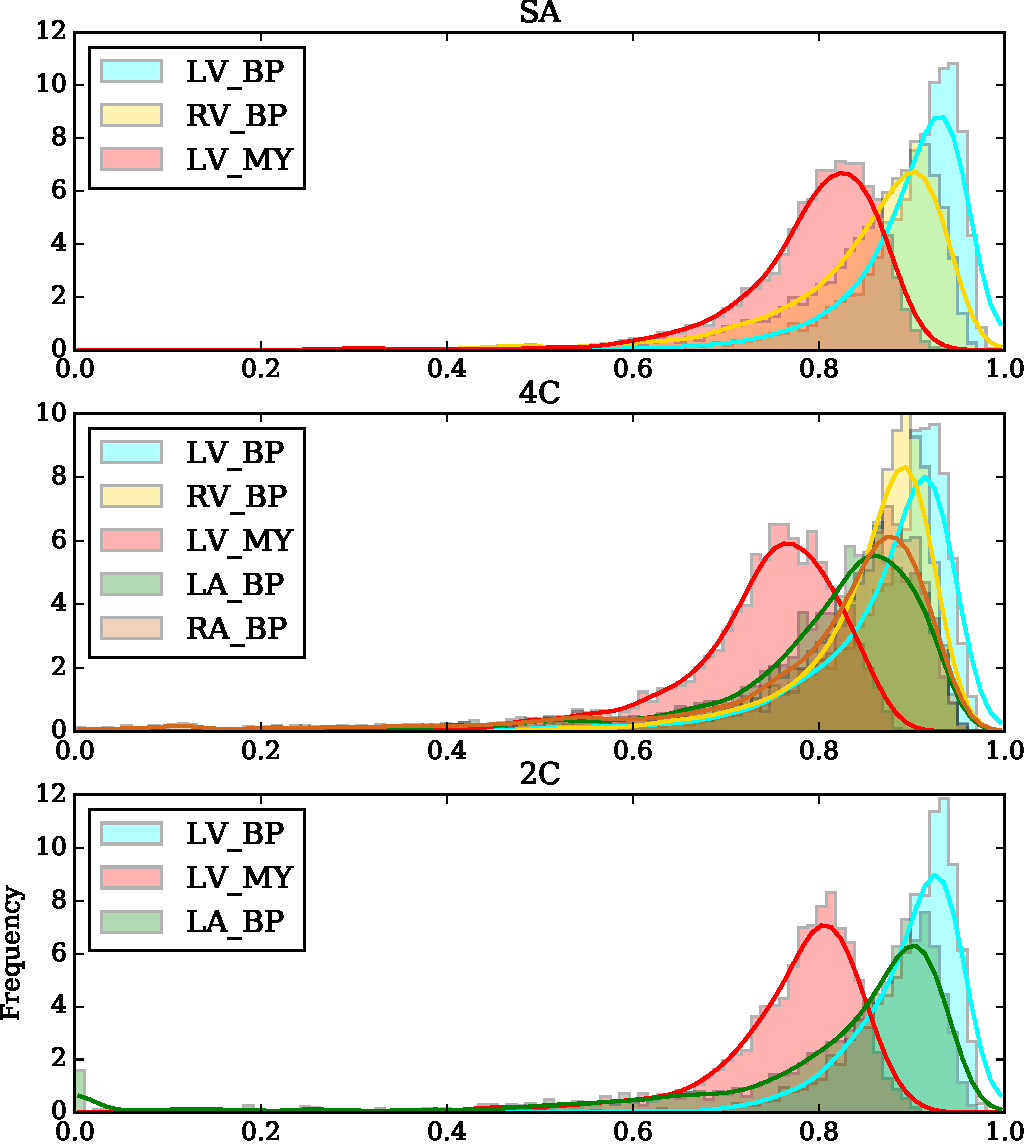
\includegraphics[width=1.0\textwidth]{./data/histograms.pdf}
\caption[\captiontitle]{\captiontitle{}. \SA{} 切面的结果最佳,\HLA{} 切面的结果最差,但是差异不大.\\
\hl{
LV\_BP:左室血池; RV\_BP:右室血池;LV\_MY:左室心肌;LA\_BP左房血池;右房血池.}
}
\label{fig:histograms}
\end{center}
\end{figure*}


考虑到不同解剖结构的分割性能会有所区别,我们将表现最好的网络 (\bestnetwork{})的每个图的的每个结构结构和每个临床切面的 \IoU{} 直方图绘制了出来,如图 \ref{fig:histograms} 所示.
在这所有的临床切面中,性能最差的是左室心肌,最好的是左室血池,其他的结构的在中等水平.
从直观上来看,相对较差的左室心肌分割性能在与边界结构的分割错误.
因此,那些有着较高的周长与面积之比的结构(如左室心肌,有着内部和外部两部分周长,也就是心内膜和心外膜)分割结果就比较差.
而左室血池的分割性能较好则有以下几个可能的因素.

\begin{itemize}
\item 左室血池周长上有高对比度的左室心肌边界.
\item 相比于其他心脏结构结构,不同被试者的左室血池差异较小.
\item 本研究使用的三个正交平面都是相对于左室来定义的;因此,不同被试者之间的左室差异也比较小.
\end{itemize}

\hl{
图 \ref{fig:roc} 为 PR 曲线,其中纵轴为成功率,成功率定义为 \IoU{} 大于阈值 $0.4$ 到 $1.0$ 的被试者百分比.
PR 曲线下面积(AUR)表示 \omeganet{} 网络的准确度.
我们还计算了失败率,即 $1 - \mathrm{success rate}$.
例如,保守估计一个 \IoU{} $< 0.9$ 时对应的失败率大约为 $1\%$.
}

\bestnetwork{} 在所有切面的正常受试者以及 \HCM{} 受试者的分割结果如图 \ref{fig:representative-results-control} 和 \ref{fig:representative-results-overt} 所示.
注意一下,分割真实值也是经过预测的参数进行了变换,这样子才能对中间帧进行插值.
网络成功地将这些例图都变换到了一个典型方向.
并且需要说明的是,心肌分割均除去了乳头肌和小梁.
而且,网络都很好的识别出了长轴图的房室瓣,这一点在以后的工作中很值得注意.

\renewcommand{\captiontitle}{PR 曲线}
\begin{figure}
\begin{center}
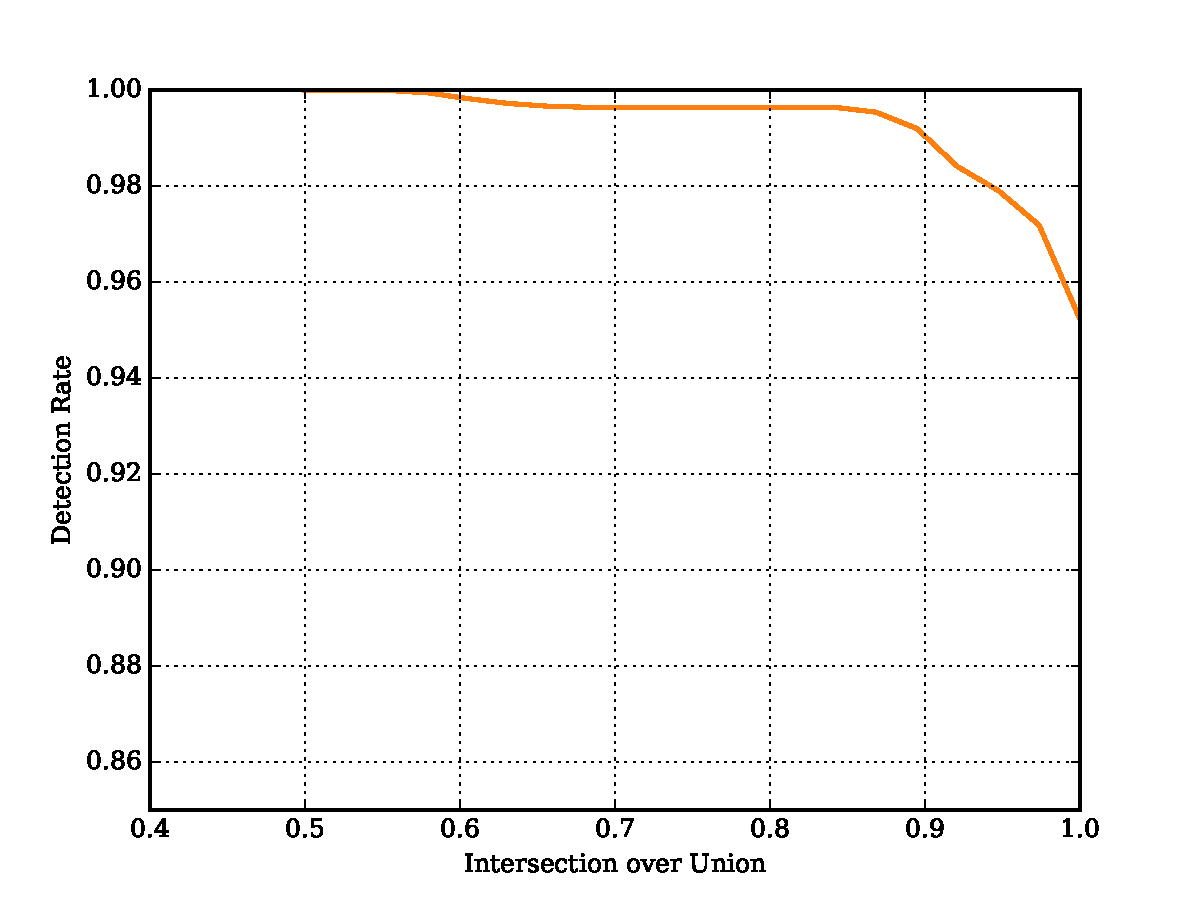
\includegraphics[width=0.5\textwidth]{./data/det_ROC_hgd_3.pdf}
\caption[\captiontitle]{\captiontitle{}.
}
\label{fig:roc}
\end{center}
\end{figure}


\renewcommand{\captiontitle}{健康受试者的分割结果}
\begin{figure*}
\begin{center}

\setlength{\tabcolsep}{1pt}

\begin{tabular}{ccccc}

\toprule
\SA{}(底层切片) & \SA{} (中间切片) & \SA{}(顶层切片) & \HLA{} & \VLA{} \\
\midrule

\multicolumn{5}{c}{未对齐方向的原始图像:$\image$} \\

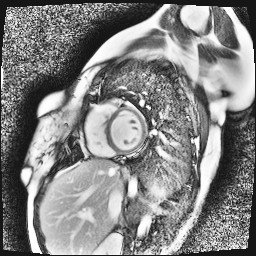
\includegraphics[width=0.19\textwidth]{./data/representative-results/control/HCMNet_2600035/00_SAX/BASE/0.png} &
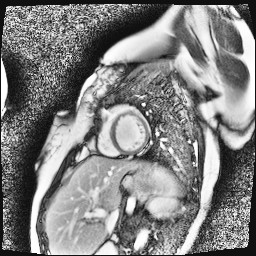
\includegraphics[width=0.19\textwidth]{./data/representative-results/control/HCMNet_2600035/00_SAX/MID/0.png} &
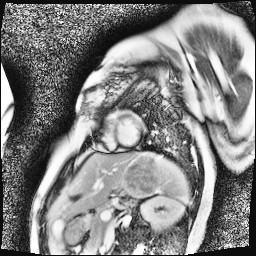
\includegraphics[width=0.19\textwidth]{./data/representative-results/control/HCMNet_2600035/00_SAX/APEX/0.png} &
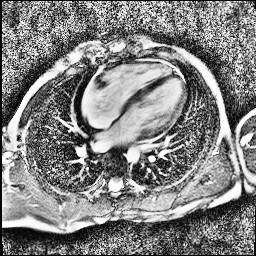
\includegraphics[width=0.19\textwidth]{./data/representative-results/control/HCMNet_1700012/01_HLA/00/0.png} &
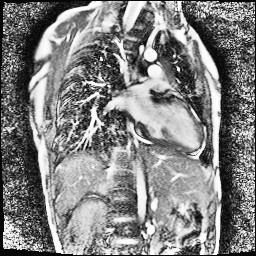
\includegraphics[width=0.19\textwidth]{./data/representative-results/control/HCMNet_1700012/02_VLA/00/0.png} \\

\multicolumn{5}{c}{结构定位} \\

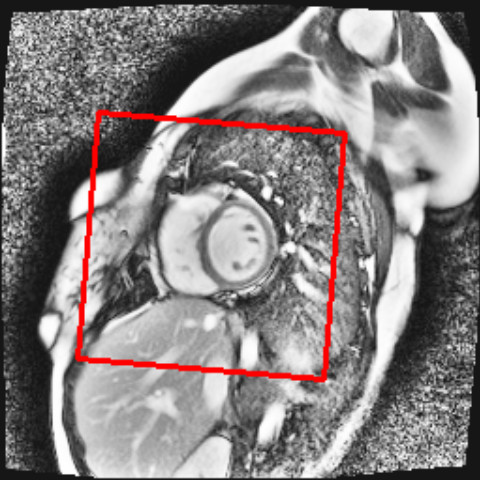
\includegraphics[width=0.19\textwidth]{./data/representative-results/control/HCMNet_2600035/00_SAX/BASE/0_bbox.png} &
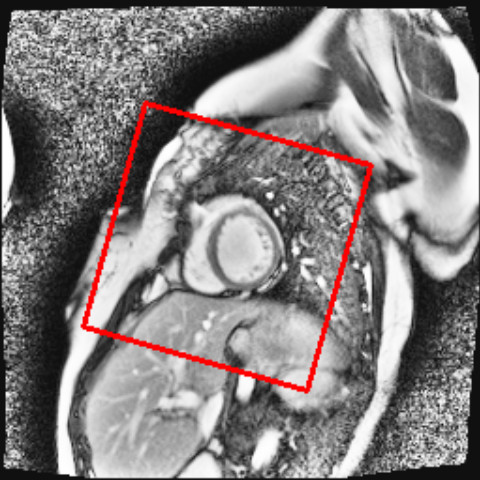
\includegraphics[width=0.19\textwidth]{./data/representative-results/control/HCMNet_2600035/00_SAX/MID/0_bbox.png} &
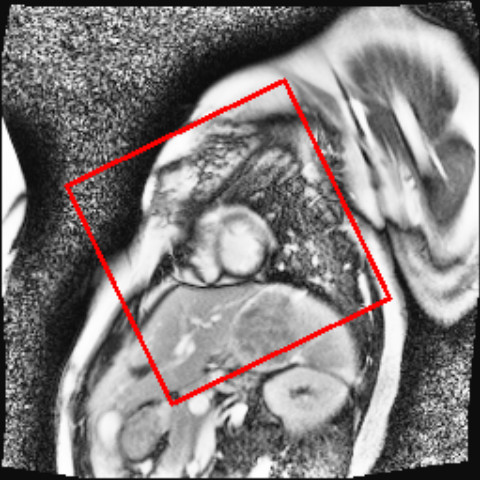
\includegraphics[width=0.19\textwidth]{./data/representative-results/control/HCMNet_2600035/00_SAX/APEX/0_bbox.png} &
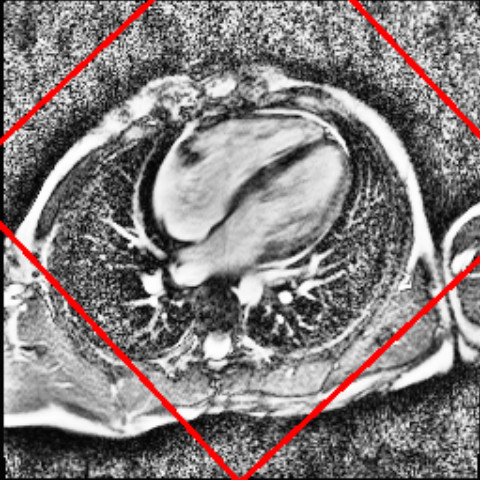
\includegraphics[width=0.19\textwidth]{./data/representative-results/control/HCMNet_1700012/01_HLA/00/0_bbox.png} &
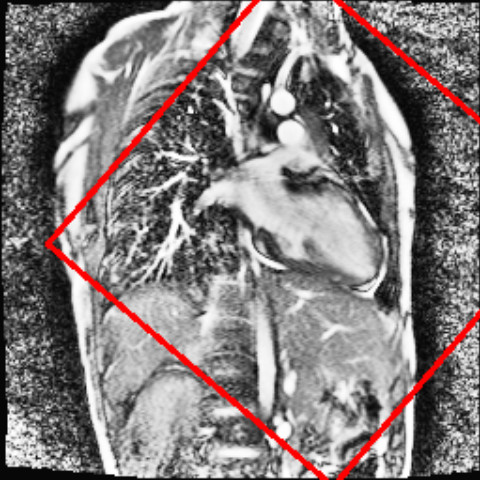
\includegraphics[width=0.19\textwidth]{./data/representative-results/control/HCMNet_1700012/02_VLA/00/0_bbox.png} \\

\multicolumn{5}{c}{在典型方向下的分割预测值:$S^\prime$} \\

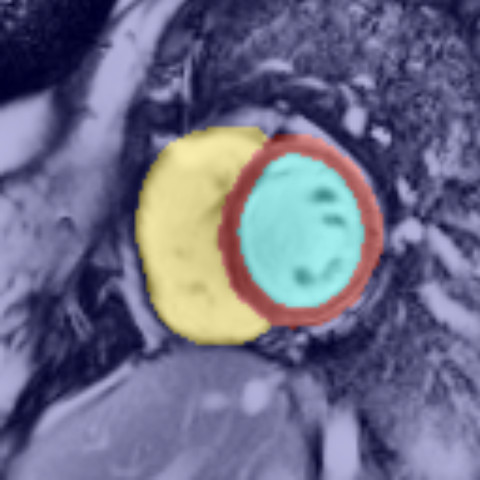
\includegraphics[width=0.19\textwidth]{./data/representative-results/control/HCMNet_2600035/00_SAX/BASE/0_pred.png} &
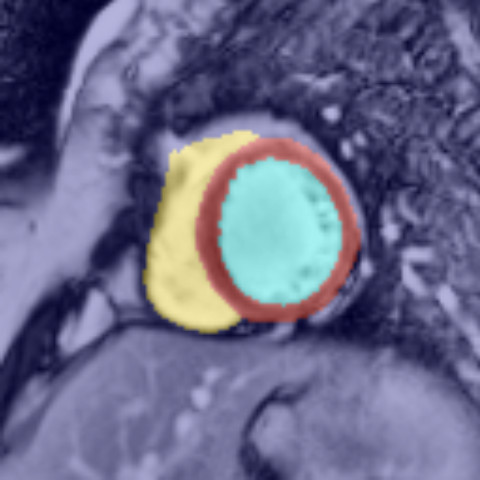
\includegraphics[width=0.19\textwidth]{./data/representative-results/control/HCMNet_2600035/00_SAX/MID/0_pred.png} &
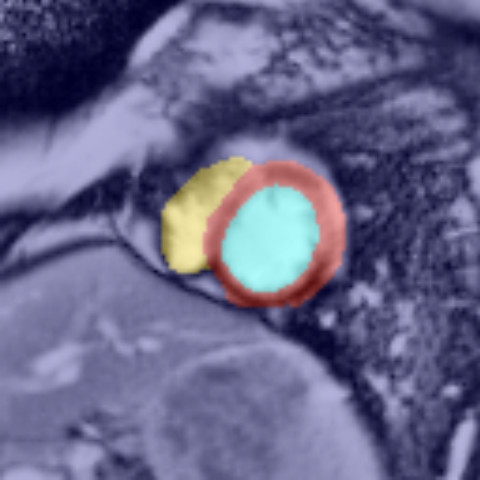
\includegraphics[width=0.19\textwidth]{./data/representative-results/control/HCMNet_2600035/00_SAX/APEX/0_pred.png} &
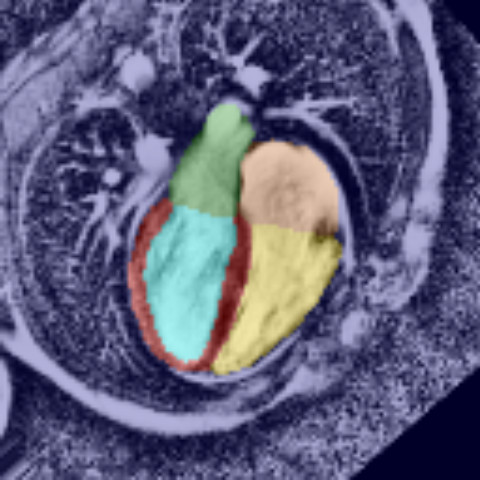
\includegraphics[width=0.19\textwidth]{./data/representative-results/control/HCMNet_1700012/01_HLA/00/0_pred.png} &
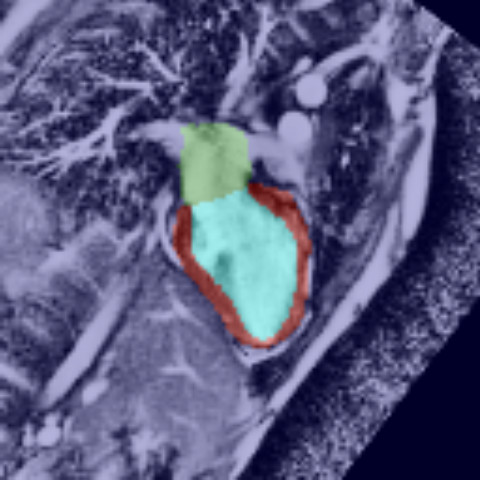
\includegraphics[width=0.19\textwidth]{./data/representative-results/control/HCMNet_1700012/02_VLA/00/0_pred.png} \\
\bottomrule

\multicolumn{5}{c}{在典型方向下的分割真实值:$\hat{S}^\prime$} \\

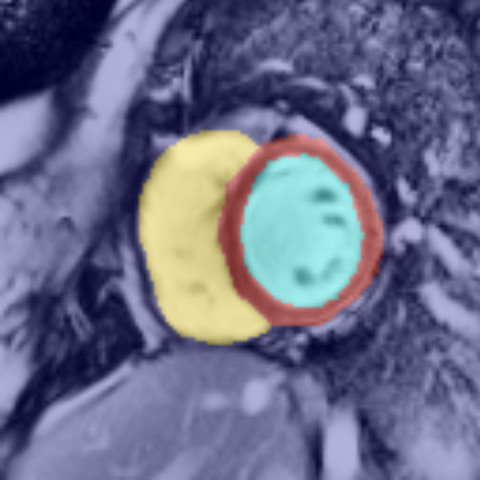
\includegraphics[width=0.19\textwidth]{./data/representative-results/control/HCMNet_2600035/00_SAX/BASE/0_gt.png} &
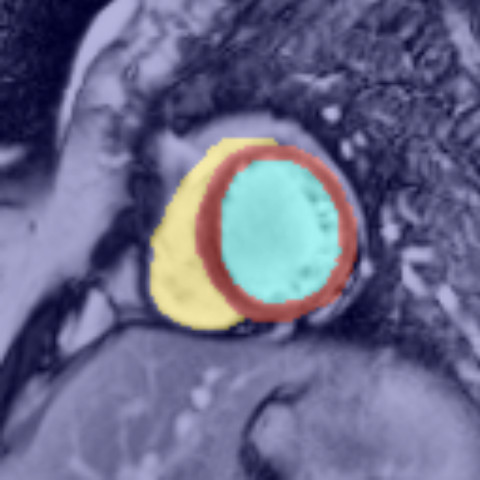
\includegraphics[width=0.19\textwidth]{./data/representative-results/control/HCMNet_2600035/00_SAX/MID/0_gt.png} &
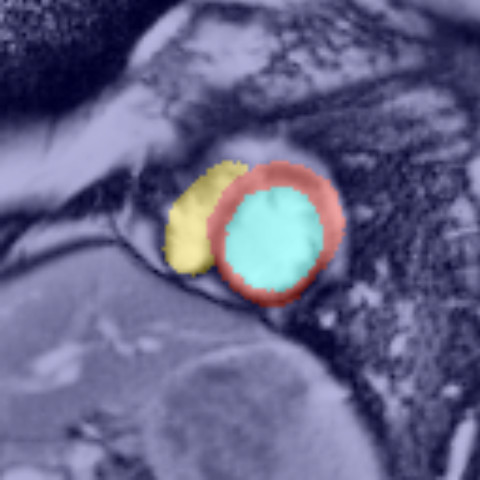
\includegraphics[width=0.19\textwidth]{./data/representative-results/control/HCMNet_2600035/00_SAX/APEX/0_gt.png} &
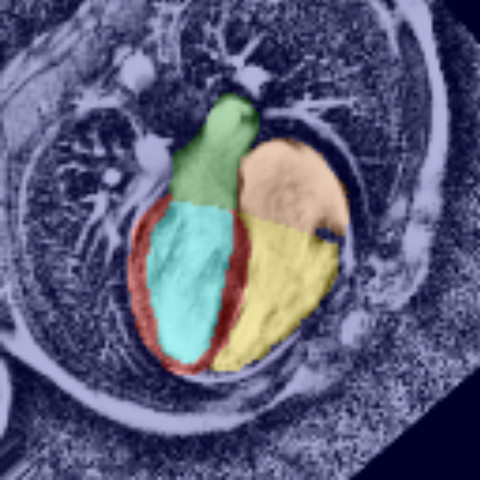
\includegraphics[width=0.19\textwidth]{./data/representative-results/control/HCMNet_1700012/01_HLA/00/0_gt.png} &
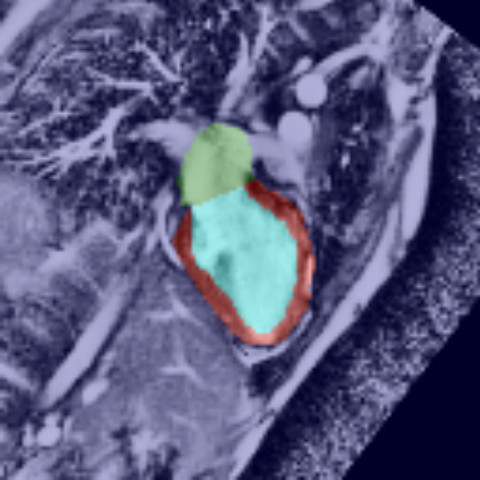
\includegraphics[width=0.19\textwidth]{./data/representative-results/control/HCMNet_1700012/02_VLA/00/0_gt.png} \\
\bottomrule

\end{tabular}

\caption[\captiontitle]{\captiontitle{}. 详细讨论请参考正文内容.}
\label{fig:representative-results-control}
\end{center}
\end{figure*}

\renewcommand{\captiontitle}{患有 \HCM{} 的患者的分割结果}
\begin{figure*}
\begin{center}

\setlength{\tabcolsep}{1pt}

\begin{tabular}{ccccc}

\toprule
\SA{}(底层切片) & \SA{}(中间切片)& \SA{}(顶层切片) & \HLA{} & \VLA{} \\
\midrule

\multicolumn{5}{c}{未对齐方向的原始图像:$\image$} \\

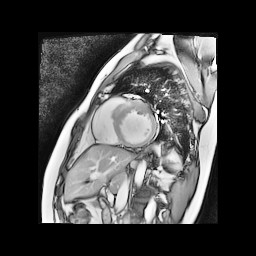
\includegraphics[width=0.19\textwidth]{./data/representative-results/overt/HCMNet_1100083/00_SAX/BASE/0.png} &
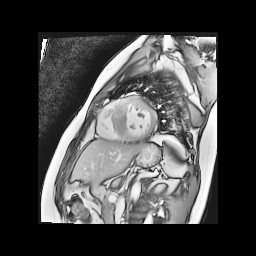
\includegraphics[width=0.19\textwidth]{./data/representative-results/overt/HCMNet_1100083/00_SAX/MID/0.png} &
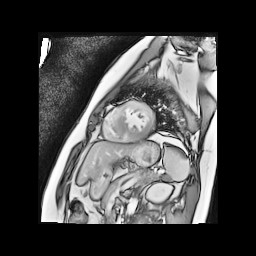
\includegraphics[width=0.19\textwidth]{./data/representative-results/overt/HCMNet_1100083/00_SAX/APEX/0.png} &
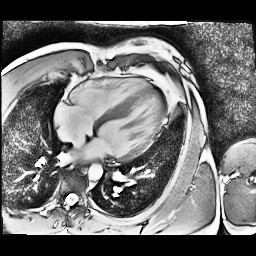
\includegraphics[width=0.19\textwidth]{./data/representative-results/overt/HCMNet_1100367/01_HLA/00/0.png} &
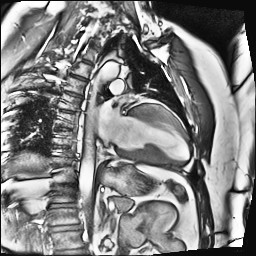
\includegraphics[width=0.19\textwidth]{./data/representative-results/overt/HCMNet_1100027/02_VLA/00/0.png} \\

\multicolumn{5}{c}{结构定位} \\

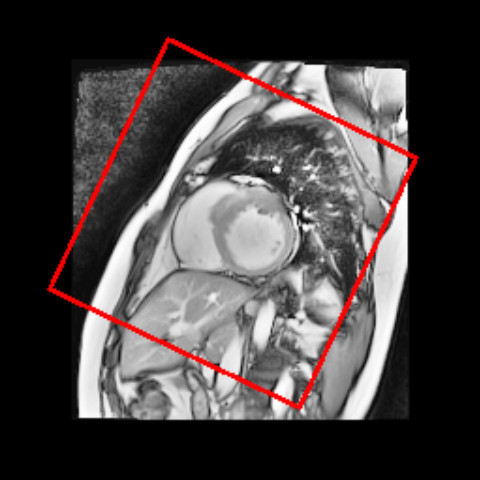
\includegraphics[width=0.19\textwidth]{./data/representative-results/overt/HCMNet_1100083/00_SAX/BASE/0_bbox.png} &
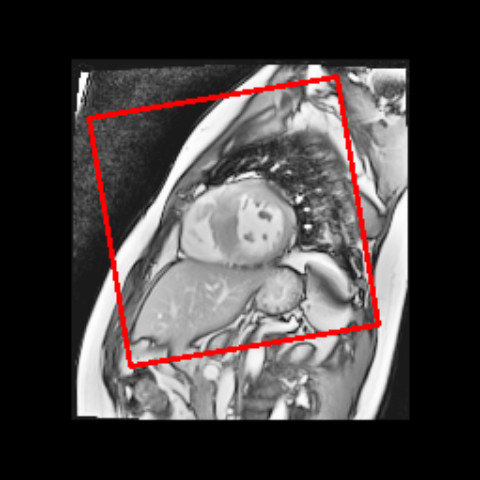
\includegraphics[width=0.19\textwidth]{./data/representative-results/overt/HCMNet_1100083/00_SAX/MID/0_bbox.png} &
\includegraphics[width=0.19\textwidth]{./data/representative-results/overt/HCMNet_1100083/00_SAX/APEX/0_bbox.png} &
\includegraphics[width=0.19\textwidth]{./data/representative-results/overt/HCMNet_1100367/01_HLA/00/0_bbox.png} &
\includegraphics[width=0.19\textwidth]{./data/representative-results/overt/HCMNet_1100027/02_VLA/00/0_bbox.png} \\

\multicolumn{5}{c}{在典型方向下的分割预测值:$S^\prime$} \\

\includegraphics[width=0.19\textwidth]{./data/representative-results/overt/HCMNet_1100083/00_SAX/BASE/0_pred.png} &
\includegraphics[width=0.19\textwidth]{./data/representative-results/overt/HCMNet_1100083/00_SAX/MID/0_pred.png} &
\includegraphics[width=0.19\textwidth]{./data/representative-results/overt/HCMNet_1100083/00_SAX/APEX/0_pred.png} &
\includegraphics[width=0.19\textwidth]{./data/representative-results/overt/HCMNet_1100367/01_HLA/00/0_pred.png} &
\includegraphics[width=0.19\textwidth]{./data/representative-results/overt/HCMNet_1100027/02_VLA/00/0_pred.png} \\
\bottomrule

\multicolumn{5}{c}{在典型方向下的分割真实值:$\hat{S}^\prime$} \\

\includegraphics[width=0.19\textwidth]{./data/representative-results/overt/HCMNet_1100083/00_SAX/BASE/0_gt.png} &
\includegraphics[width=0.19\textwidth]{./data/representative-results/overt/HCMNet_1100083/00_SAX/MID/0_gt.png} &
\includegraphics[width=0.19\textwidth]{./data/representative-results/overt/HCMNet_1100083/00_SAX/APEX/0_gt.png} &
\includegraphics[width=0.19\textwidth]{./data/representative-results/overt/HCMNet_1100367/01_HLA/00/0_gt.png} &
\includegraphics[width=0.19\textwidth]{./data/representative-results/overt/HCMNet_1100027/02_VLA/00/0_gt.png} \\
\bottomrule

\end{tabular}

\caption[\captiontitle]{\captiontitle{}.详细讨论请参考正文内容.}
\label{fig:representative-results-overt}
\end{center}
\end{figure*}


\subsubsection{变换参数}

\renewcommand{\captiontitle}{变换误差}
\begin{sidewaysfigure*}
\begin{center}
\includegraphics[width=1.0\textwidth]{./data/matrix-loss.png}
\caption[\captiontitle]{\captiontitle{}.
我们给出了变换参数的预测值与真实值之间的相关系数图(上)和 Bland-Altman 图(下).
\SA{}、\HLA{} 和 \VLA{} 误差分贝用橙色、绿色和紫色点表示(所有的点都做了半透明处理,以方便查看).
在相关系数图中,最佳的拟合线用黑色实线表示,理想的线条($y = x$)用灰色的虚线表示.
我们也给出了拟合线的公式和皮尔森相关系数 $R$.
而在 Bland-Altman 图中,误差均值用黑色水平实线表示,$\pm 1.96$ 的标准差界线用灰色水平虚线表示.
}
\label{fig:matrix-loss}
\end{center}
\end{sidewaysfigure*}



我们通过相关系数和 Bland Altman 图(见图 \ref{fig:matrix-loss})来比较参数真实值与性能最好的网络(\bestnetwork{})进行比较.
需要指出的是,变换参数的真实值,特别是旋转和缩放,并不是在所有切面上均匀分布的.
非随机的旋转应该是由以下原因导致的,包括病人与扫描器的相对位置,扫查平面的流程,心脏和胸腔的位置以及不同扫查平面之间的关系都是非随机的;而非随机的缩放则可能是因为在每一切面中结构结构的可视范围不同.

水平平移,垂直平移和旋转参数的预测值与真实值是高度相关的($R \approx~0.95$, $p < 0.0001$),而预测参数相比于真实值都是略有低估了($\approx~0.87$).
从 Bland-Altman 图中看来,系统的偏移并不明显;$95\%$ 的平移误差在 $\pm 0.07$(以归一化后的图像坐标计算)以内,而 $95\%$ 的旋转误差在 $\pm 0.63$ 以内(以弧度计算).
在那些 $5\%$ 的离群值里,大部分都集中在长轴切面(\HLA{} 和 \VLA{}).
考虑到每个病人都提供了三个短轴切面,而只有两个长轴切面,这一点应该不太令人感到惊讶.

比起平移和旋转,缩放的预测值与真实值的相关系数略低,但依然是不错的($R = 0.88$, $p < 0.0001$);缩放的预测值比起真实值依然是低估了($s = 0.71\hat{s} + 0.16$).
注意到在网络大约有个 $\hat{s} = 0.7$ 的性能下降.
这也许指明了上下文信息的重要性.
当然,也有可能是由于样本量步骤导致的.

\subsubsection{失败的例子}

\renewcommand{\captiontitle}{\CNN{} 分割错误例子}
\begin{figure*}
\begin{center}

\setlength{\tabcolsep}{1pt}

\begin{tabular}{cccc}

\toprule
\SA{}(顶层切片) & \SA{}(顶层切片) & \HLA{} & \VLA{} \\
\midrule

\multicolumn{4}{c}{未对齐方向的原始图像:$\image$} \\

\includegraphics[width=0.19\textwidth]{./data/failures/HCMNet_2000062/00_SAX/9/9.png} &
\includegraphics[width=0.19\textwidth]{./data/failures/HCMNet_2400044/00_SAX/2/5.png} &
\includegraphics[width=0.19\textwidth]{./data/failures/HCMNet_2600079/01_HLA/00/0.png} &
\includegraphics[width=0.19\textwidth]{./data/failures/HCMNet_2600079/02_VLA/00/0.png} \\

\multicolumn{4}{c}{结构定位} \\

\includegraphics[width=0.19\textwidth]{./data/failures/HCMNet_2000062/00_SAX/9/9_bbox.png} &
\includegraphics[width=0.19\textwidth]{./data/failures/HCMNet_2400044/00_SAX/2/5_bbox.png} &
\includegraphics[width=0.19\textwidth]{./data/failures/HCMNet_2600079/01_HLA/00/0_bbox.png} &
\includegraphics[width=0.19\textwidth]{./data/failures/HCMNet_2600079/02_VLA/00/0_bbox.png} \\

\multicolumn{4}{c}{在典型方向下的分割预测值:$S^\prime$} \\

\includegraphics[width=0.19\textwidth]{./data/failures/HCMNet_2000062/00_SAX/9/9_pred.png} &
\includegraphics[width=0.19\textwidth]{./data/failures/HCMNet_2400044/00_SAX/2/5_pred.png} &
\includegraphics[width=0.19\textwidth]{./data/failures/HCMNet_2600079/01_HLA/00/0_pred.png} &
\includegraphics[width=0.19\textwidth]{./data/failures/HCMNet_2600079/02_VLA/00/0_pred.png} \\
\bottomrule

\multicolumn{4}{c}{在典型方向下的分割真实值:$\hat{S}^\prime$} \\

\includegraphics[width=0.19\textwidth]{./data/failures/HCMNet_2000062/00_SAX/9/9_gt.png} &
\includegraphics[width=0.19\textwidth]{./data/failures/HCMNet_2400044/00_SAX/2/5_gt.png} &
\includegraphics[width=0.19\textwidth]{./data/failures/HCMNet_2600079/01_HLA/00/0_gt.png} &
\includegraphics[width=0.19\textwidth]{./data/failures/HCMNet_2600079/02_VLA/00/0_gt.png} \\
\bottomrule

\end{tabular}

\caption[\captiontitle]{\captiontitle{}.详细讨论参考正文.}
\label{fig:failure}
\end{center}
\end{figure*}


我们也观察到偶然分割失败的例子,其中一些例子如图 \ref{fig:failure} 所示.
每一个失败的例子都有一两个可以解释的原因.
最左一栏的例子为一个严重心肌肥大的病人的 \SA{} 切面.
这样的例子是数据集中比较罕见的,所以导致网络分割结果很差.
第二栏的例子是另一个病人的 \SA{} 切面,其右室被错误的分割.
这个图中的灰度整体比较低,导致经过直方图均衡处理之后对比度太高.
第三和第四栏的图中扫描分辨率太高,以致于心脏占了整个图的大部分区域,进而导致缺少上下文信息.
这里例子中的糟糕分割结果都是由于图像没能正确地变换到一个典型方向.
然而,需要强调的是,这些事后诸葛亮的分析;我们并不能直接给出这些特征与分割失败之间的关系.

\subsection{2017 MICCAI \miccaidata{} 数据集}
\renewcommand{\captiontitle}{在 2017 MICCIA \miccaidata{} 数据集上的分割准确率}
\begin{table*}
\hl{
\begin{center}
\begin{tabular}{lccc} \hline
\toprule
结构           & 左室血池 & 右室血池 & 左室心肌 \\
\midrule
\multicolumn{4}{c}{Jaccard 系数(\IoU{})} \\
\midrule
\omeganet{}         & \textbf{\ACDCONJLVBP{}}  & \textbf{\ACDCONJRVBP{}}  & \ACDCONJLVMY{}           \\
\citet{Isensee2018} & \ACDCFINJLVBP{}          & \ACDCFINJRVBP{}          & \textbf{\ACDCFINJLVMY{}} \\
\citet{Isensee2017} & \ACDCFIOJLVBP{}          & \ACDCFIOJRVBP{}          & \ACDCFIOJLVMY{}          \\
\midrule
\multicolumn{4}{c}{Dice 系数} \\
\midrule
\omeganet{}         & \textbf{\ACDCONDLVBP{}}  & \textbf{\ACDCONDRVBP{}}  & \ACDCONDLVMY{}           \\
\citet{Isensee2018} & \ACDCFINDLVBP{}          & \ACDCFINDRVBP{}          & \textbf{\ACDCFINDLVMY{}} \\
\citet{Isensee2017} & \ACDCFIODLVBP{}          & \ACDCFIODRVBP{}          & \ACDCFIODLVMY{}          \\
\bottomrule
\end{tabular}
\caption[\captiontitle{}]{
\hl{
\captiontitle{}.
\miccaidata{} 挑战的分割准确率用 Dice 系数计算,其他的地方使用 \IoU{} 计算;因此这里把两个都计算出来了.
(提示,$\mathrm{Dice} = 2 * \mathrm{\IoU{}} / (1 + \mathrm{\IoU{}})$)
我们给出了 \omeganet{} 网络 B 的结果;\citet{Isensee2017} 发表在 STACOM 上的结果;以及 \citet{Isensee2018} 在 \url{arxiv.org} 上预发表的结果.
每一前景类别的最佳结果用加粗字体标出.
}
}
\label{tab:acdc}
\end{center}
}
\end{table*}

\citet{Isensee2017} 在 \miccaidata{} 排行榜上取得了最佳的成绩;他们 \citep{Isensee2018} 还预发表 \footnote{https://arxiv.org/abs/1707.00587v2} 了一个更好的结果.
为了与他们的结果比较,我们在 MICCAI \miccaidata{} 上从头开始训练了 \omeganet{} 网络 B,使用五折交叉验证,并且每一个受试者的数据仅出现在其中一折中.
\omeganet{} 模型,\citet{Isensee2017} 以及 \citet{Isensee2018} 的分割准确率对比如表 \ref{tab:acdc} 所示.
相比于 \citet{Isensee2017},我们的结果中每一类的 \IoU{} 都更高:左室血池($\ACDCONJLVBP{}$ vs $\ACDCFIOJLVBP{}$),右室血池($\ACDCONJRVBP{}$ vs $\ACDCFIOJRVBP{}$)和左室心肌($\ACDCONJLVMY{}$ vs $\ACDCFIOJLVMY{}$).
相比于 \citet{Isensee2018},我们的左室血池($\ACDCONJLVBP{}$ vs $\ACDCFINJLVBP{}$)和右室血池($\ACDCONJRVBP{}$ vs $\ACDCFINJRVBP{}$)的 \IoU{} 更高,但是左室心肌($\ACDCONJLVMY{}$ vs $\ACDCFINJLVMY{}$)的较低.


%%%%%%%%%%%%%%%%%%%%%%%%%%%%%%%%%%%%%%%%%%%%%%%%%%%%%%%%%%%%%%%%%%%%%%%%%%%%%%%%
%% Discussion
%%%%%%%%%%%%%%%%%%%%%%%%%%%%%%%%%%%%%%%%%%%%%%%%%%%%%%%%%%%%%%%%%%%%%%%%%%%%%%%%

\section{讨论} \label{discussion}

本文中,我们提出了 \omeganet{}:一个全新的深度卷积神经网络结构,可以用于定位、方向对齐和分割.
我们将该网络应用到了全自动的全心分割,同时将图像变换到一个典型方向,从而大大地降低了 \SSFP{} \CMR{} 图像的分析难度.
无需先验知识,我们从头开始端到端的训练了该网络,用来对三个切面(\SA{}、\HLA{}和\VLA{})的五个前景类别(心脏的四个心腔加上左室心肌)进行分割.
从解剖的角度来看,这个数据集是高度异质的,包含了健康的受试者和肥厚性心肌病患者.
数据采集自10个医疗中心,包括 1.5-T 和 3-T 核磁共振图像.
在交叉验证实验中,网络在变换参数预测与分割任务中均表现良好.

\hl{
\omeganet{} 也在 2017 MICCAI \miccaidata{} 公开数据集的两个类别中的分割任务中取得最好的成绩.
相比于我们内部的 HCMNet 数据集,\miccaidata{} 包含了更多的 \LV{} 和 \RV{} 病例,但是只有一个临床切面,和更少的前景类别.
而且,HCMNet 数据集是多中心研究的结果,而\miccaidata{} 则来自单中心.

之前最好的分割 \citep{Isensee2017,Isensee2018} 同时集成了 2D 和 3D \UNet{} 结构,为堆叠的视频序列进行优化.
他们的方法也因此不适用于 \HLA{} 和 \VLA{} 切面,因为这些切面通常只采集一个静态图.
因此,我们的 \omeganet{} 不仅分割性能比 \citet{Isensee2018} 好,而且也更加通用,同时还能提供 \citep{Isensee2017} 所不具备的定位和方向对齐信息.
}

本研究在这么四个方面具有创新性.
第一,这个网络预测了三个切面中的五个前景类别,如 \citep{Vigneault2017} 所言,这个任务是更加困难和棘手的.
第二,我们用一个空间变换网络模块 \citep{Jaderberg2015} 来将每个切面都变换到一个典型方向去.
\hl{
\CNN{} 既不是旋转不变的也不是尺度不变的.
从技术上来说,我们是可以通过获取一个足够大的数据集,里面包含了各种可能的旋转变化,从而克服这个缺点.
但是,生物医学图像的获取和标注都是十分昂贵和耗时的,这也就催生了我们的这个设计.
通过将最后的细分割的输入图像进行标准化的变换,我们简化了网络的设计,同时还模拟了医师的操作.
}
第三,这个网络结构启发自 \citet{Viola2001} 的级联分类模型,我们使用 \UNet{} $0$ 来进行粗分割(为了预测变换参数),然后变换后的图像被送入细分割模块(\UNet{}s $1$,$2$和$3$).
\hl{
最后,\omeganet{} 从其本身的设计出发,提供了一定的可解释性,包括中间层的输出(粗分割结果和变换参数)和最后的细分割.
这样子,我们的网络比起 \UNet{} 结构提升了复杂度和可预测的信息,但是无寻担心 CNN 无法解释的黑盒子问题.
}

尽管该数据集包含了三个切面,也包含了健康受试者和有左心疾病的患者,我们还是可以将该数据集扩充到其他更加通用的场景.
首先,其他常用的心脏切面(例如轴面、三腔和右室长轴面)应该在未来的工作中添加到数据集中来.
另外,在其他的 \CMR{} 图像序列(例如灰度超声心动图)或者模态(比如心脏 CT 和超声心动图)的测试也很值得尝试.
而且,将这个网络应用到其他也需要定位、重新对齐方向和分割的生物医学图像任务中也是很有意思的,比如胎儿影像.
\hl{
最后,我们希望 \omeganet{} 能在其他需要多个临床切面分割的应用中也能有效应用,例如 \CMR{} 运动校正和切面配准 \citep{Sinclair2017}.
}

\omeganet{} 还有很多可以优化的地方.
例如,我们可以训练网络对单帧图像进行分割,而无需空间或者时间的上下文信息;修改网络结构以共享时间序列和空间切片的信息,从而提升网络性能.
E-Net(``Efficient Net'')提供了一个改进版的 \UNet{} 模块,它能有效地提升计算效率和降低显存使用,同时还能保证准确率 \citep{Paszke2016};这些经验已经有效地应用到了心脏的分割 \citep{Lieman-Sifry2017},理论上来说应该也能应用到这里.


%%%%%%%%%%%%%%%%%%%%%%%%%%%%%%%%%%%%%%%%%%%%%%%%%%%%%%%%%%%%%%%%%%%%%%%%%%%%%%%%
%% Summary
%%%%%%%%%%%%%%%%%%%%%%%%%%%%%%%%%%%%%%%%%%%%%%%%%%%%%%%%%%%%%%%%%%%%%%%%%%%%%%%%

\section{总结} \label{summary}


我们已经展示了 \omeganet{}(Omega-Net):一个全新的 \CNN{} 网络结构,同时完成定位、变换到一个典型方向和语义分割.
首先,我们对输入图像进行粗分割;然后我们利用粗分割学习到的特征进行变换参数的预测,利用这些参数可以将输入图像变换到一个典型方向;最后,我们对变换后的图像进行细分割.
我们在两个不同的数据集上从头开始端到端训练了网络.
在 HCMNet 数据集上,我们训练 \omeganet{} 来预测三个切面的五个前景类别,这个任务比起以前的任务都更加具有挑战性.

网络在健康受试者和患有严重左室心脏病的患者的数据上表现都非常好.
所有的 \omeganet{} 网络变种都在公开数据集上从头开始训练,并在三个分割类别中的两个表现最佳.
我们相信这个网络结构比起以前的网络更加优秀,并且在生物医学图像分割任务中还具有通用性.




%%%%%%%%%%%%%%%%%%%%%%%%%%%%%%%%%%%%%%%%%%%%%%%%%%%%%%%%%%%%%%%%%%%%%%%%%%%%%%%%
%% Acknowledgements
%%%%%%%%%%%%%%%%%%%%%%%%%%%%%%%%%%%%%%%%%%%%%%%%%%%%%%%%%%%%%%%%%%%%%%%%%%%%%%%%

\section*{致谢} \label{acknowledgements}

D.M. Vigneault 得到了 NIH-Oxford 学者计划和 NIH 学院研究计划的资助.
W. Xie 获得了 Google DeepMind 奖学金和 EPSRC Programme Grant Seebibyte EP/M013774/1 的资助.


%%%%%%%%%%%%%%%%%%%%%%%%%%%%%%%%%%%%%%%%%%%%%%%%%%%%%%%%%%%%%%%%%%%%%%%%%%%%%%%%
%% References
%%%%%%%%%%%%%%%%%%%%%%%%%%%%%%%%%%%%%%%%%%%%%%%%%%%%%%%%%%%%%%%%%%%%%%%%%%%%%%%%

\section*{参考文献} \label{references}

\bibliography{citations}

\end{document}

